\pdfoutput=1
\documentclass[11pt]{amsart}
\usepackage{amsmath,amssymb,amsthm,mathtools,mathrsfs}
\usepackage[margin=1.2in]{geometry}
\usepackage{graphicx,booktabs,adjustbox,tikz}
\usetikzlibrary{arrows.meta,positioning}
\usepackage{xcolor}
\usepackage[colorlinks=true,linkcolor=blue,citecolor=blue,urlcolor=blue]{hyperref}
\hypersetup{pdfauthor={Bernd Johannes Wuebben},
 pdftitle={Metric response and Hermitian Yang--Mills flow for two-step extensions}}
\setlength{\emergencystretch}{2em}
\newtheorem{theorem}{Theorem}[section]
\newtheorem{proposition}[theorem]{Proposition}
\newtheorem{lemma}[theorem]{Lemma}
\newtheorem{corollary}[theorem]{Corollary}
\theoremstyle{definition}
\newtheorem{definition}[theorem]{Definition}
\newtheorem{example}[theorem]{Example}
\newtheorem{question}[theorem]{Question}
\theoremstyle{remark}
\newtheorem{remark}[theorem]{Remark}
\newcommand{\RR}{\mathbb R}
\newcommand{\CC}{\mathbb C}
\newcommand{\PP}{\mathbb P}
\newcommand{\cO}{\mathcal O}
\newcommand{\HH}{\mathcal H}
\newcommand{\cK}{\mathcal K}
\newcommand{\db}{\bar\partial}
\newcommand{\End}{\operatorname{End}}
\newcommand{\Hom}{\operatorname{Hom}}
\newcommand{\Ext}{\operatorname{Ext}}
\newcommand{\tr}{\operatorname{tr}}
\newcommand{\rk}{\operatorname{rk}}
\newcommand{\diag}{\operatorname{diag}}
\newcommand{\ad}{\operatorname{ad}}
\newcommand{\id}{\operatorname{id}}
\newcommand{\one}{\mathbf1}
\title[Metric response and Hermitian Yang--Mills flow]{Metric response and Hermitian Yang--Mills flow\\for two-step extensions}
\author{Bernd Johannes Wuebben}
\subjclass[2020]{53C07 (primary); 53C55, 58J35, 58J50 (secondary)}
\keywords{Hermitian--Einstein metric, Hermitian Yang--Mills flow,
 slope stability, vector bundle extension, graph Laplacian, metric variation}
\date{October 27, 2026}
\begin{document}
\begin{abstract}
For two-step extensions of pairwise nonisomorphic stable bundles on a
compact Kähler manifold, we quantify the degeneration of
Hermitian--Einstein metrics and Hermitian Yang--Mills flow near
intersecting slope-stability walls. We assume equal slopes at the
reference form and connected support for the extension class.
When the centered slopes provide full local parameters, every singular
value of the trace-free part of \(H^{-1}dH\), for the
Hermitian--Einstein metric \(H\), is relatively asymptotic to the
reciprocal of a nonzero eigenvalue of a weighted extension-graph
Laplacian. The comparison uses rank-weighted slope and normalized
\(L^2\) norms and remains uniform for arbitrarily separated positive
stability margins. We also construct a finite-dimensional invariant
manifold of the flow and compare its solutions with flows from any
smooth family of initial metrics. For each tolerance, one late time
and then one parameter neighborhood give multiplicative metric
comparison, up to a constant scalar, and relative accuracy for every
small endomorphism Dolbeault eigenvalue for all subsequent times.
The comparison applies in the stable, semistable and unstable regimes.
In the two-factor case, we determine a uniform asymptotic profile for
the smallest eigenvalue across the wall, including exponential decay
on the unstable side.
An application to explicit weak Fano toric tangent bundles connects
nonsimplicial stability chambers, metric response and flow on the
same bundles.
\end{abstract}
\maketitle
\enlargethispage{5pt}


% ============================================================
% section_01_introduction.tex
% ============================================================
\section{Introduction}\label{sec01:intro}

The Kobayashi--Hitchin correspondence decides the existence of a
Hermitian--Einstein metric from slope stability. Near a stability
wall the limiting graded bundle has additional automorphisms, and
the metric equation loses invertibility in the corresponding
directions. We ask for a quantitative description that remains
valid when several wall distances vanish at unrelated rates.
The relevant finite operator is a weighted extension-graph
Laplacian. This paper determines the singular values of the
intrinsic metric derivative, separates the singular part of the
linear inverse, and proves actual-flow comparisons with a finite
evolution. A final theorem connects these statements on one family
of genuine toric tangent bundles.

Consider a fixed holomorphic two-step extension
\[
 0\longrightarrow\bigoplus_{i\in I}F_i\longrightarrow E
     \longrightarrow\bigoplus_{j\in J}F_j\longrightarrow0
\]
on a compact connected Kähler manifold \(X\) of complex dimension
\(n\). The \(m\) factors are
locally free, pairwise nonisomorphic, and stable with equal slope
at the reference form \(\omega_0\). There is an edge \(j\to i\)
for every nonzero component of its fixed extension class; assume
the underlying bipartite graph is connected. Let \(\omega_s\)
be a smooth finite-dimensional Kähler family, \(r_v=\rk F_v\),
\(M=\diag(r_v)\), and \(D_e=e_i-e_j\). With smoothly continued
factor HE metrics and harmonic representatives \(\beta_{e,s}\), put
\begin{equation}\label{eq01:data}
 \begin{gathered}
 V_s=\int_X\omega_s^n/n!,\qquad
 \kappa_v(s)=\frac{2\pi c_1(F_v)[\omega_s]^{n-1}}
                  {(n-1)!V_sr_v},\qquad
 \kappa_E=\frac{\sum_vr_v\kappa_v}{\sum_vr_v},\\
 b_v=-r_v(\kappa_v-\kappa_E),\qquad
 c_e(s)=\|\beta_{e,s}\|_{L^2}^2/V_s>0.
 \end{gathered}
\end{equation}
For \(b\in D\RR_{>0}^{E(\Gamma)}\), exponential balancing means
\begin{equation}\label{eq01:balance}
 k_e=c_e(s)e^{(D^Tx^0)_e},\quad Dk=b,\quad
 \sum_vr_vx_v^0=0,\qquad\sigma=\sum_ek_e.
\end{equation}
It has a unique solution. Denote the positive eigenvalues of
\(M^{-1/2}D\diag(k)D^TM^{-1/2}\), in increasing order, by
\(\nu_1(k),\ldots,\nu_{m-1}(k)\).
For a nonempty proper vertex subset \(C\), let \(\partial C\)
be the edges joining \(C\) to its complement, and define its
cut capacity and normalized capacity by
\[
 \operatorname{cap}_k(C)=\sum_{e\in\partial C}k_e,\qquad
 \frac{\operatorname{cap}_k(C)}{\sum_ek_e}.
\]
These definitions apply to any positive conductance array used below.
The independent stationary theorem in \cite{wuebben2026uniform}
constructs actual HE metrics and gives every complex small
endomorphism eigenvalue relatively by this operator. We restate
its hypotheses and normalizations in Section~\ref{sec02:stationary}.

\begin{theorem}[Intrinsic metric response]\label{thm01:response}
Suppose the centered slope map \(s\mapsto b(s)\) has full rank
\(m-1\) at the wall. Use a smooth chart \(s=s(b,\zeta)\), with
bounded first derivatives near the wall, and hold \(\zeta\) fixed.
For the actual HE metric \(H_s\) in the local stable chamber,
consider
\[
 \dot b\longmapsto\mathscr D_s\dot b
            =(H_s^{-1}\partial_{\dot b}H_s)_0.
\]
The input norm is \(\|\dot b\|_{M^{-1}}^2=\sum_v\dot b_v^2/r_v\).
The output is a real \(H_s\)-Hermitian pointwise trace-free
endomorphism, with norm squared
\(V_s^{-1}\int_X\tr(A^2)\,dV_s\). Its decreasing singular values
obey
\begin{equation}\label{eq01:response}
 s_j(\mathscr D_s)=\frac{1+O(\sigma)}{\nu_j(k(s,b))},
 \qquad 1\le j<m.
\end{equation}
The coefficient is one. The error constant remains uniform as
positive normalized cut capacities or ratios of positive graph
eigenvalues tend to zero, including repeated eigenvalues and
approaches to intersecting chamber faces. The metric tangent is intrinsic;
it is not the derivative of a fixed-frame matrix logarithm.
\end{theorem}

Theorem~\ref{thm03:inverse} gives the accompanying exact inverse and
positive-resolvent decomposition. Its finite Schur form agrees with
the graph form up to a relative \(O(\sigma)\) error, and its
complementary inverse is uniformly regular
in fixed Sobolev norms in the scaled harmonic presentation.
Theorem~\ref{thm04:response} proves \eqref{eq01:response} from an
exact differentiation identity, rather than differentiating a
\(C^0\) approximation. Neither conclusion is a nonlinear choice
of gauge on a quotient moduli space.
For the general two-step extension, Theorem~\ref{thm08:flow} also
gives metric and relative spectral comparison for prescribed HYM
flows at stable, wall and unstable nearby parameters. Its parameter
neighborhood is chosen after the comparison time.

\subsection*{One geometric family and the synthesis theorem}
For \(k\ge1\), put \(d=2k\), \(n=d+2\), and, with quotient
projectivization, set
\[
 B=(\PP^1)^d,\qquad L=\cO_B(1^k,-1^k),\qquad
 X_k=\PP_B(\cO\oplus L)\times_B\PP_B(\cO\oplus L).
\]
Write \(\pi:X_k\to B\). Let \(h_j\) be the pulled-back hyperplane
class of the \(j\)-th base factor, and let \(\xi_i\) be the first
Chern class of the tautological quotient line bundle from the
\(i\)-th projective-bundle factor. Put \(\ell=c_1(L)\),
\(\eta_i=\xi_i-\ell/2\), and define the line bundles
\[
 R_i=\cO_{X_k}(2\xi_i)\otimes\pi^*L^{-1},\qquad
 Q_j=\pi^*\cO_B(2h_j).
\]
Their Chern classes, in vertex order \((R_1,R_2,Q_1,\ldots,Q_d)\),
are \(C=(2\eta_1,2\eta_2,2h_1,\ldots,2h_d)\).
The equality poset \(K_{2,d}\) has two minimal elements, \(d\)
maximal elements, and every minimal element below every maximal
element. Its order ideals index the invariant saturated tangent
subsheaves having the same slope as the tangent bundle at the wall.
For a Hermitian metric \(h\), let \(F_h\) denote its Chern curvature
and \(K_{h,\omega}=i\Lambda_\omega F_h\) its mean curvature.
Use the smoothly varying line-factor metrics \(h_{v,s}\), and put
\(h_{0,s}=\bigoplus_vh_{v,s}\). For the flow statement, write
\(u=\Psi(s,t)\) for the parabolic invariant graph constructed in
Section~\ref{sec06:graph}, where \(t=(t_{ij})\) is the vector of
extension amplitudes. Its diagonal gauge velocity is denoted
\(A_s(t)\): the corresponding positive diagonal gauge solves
\(\dot g_sg_s^{-1}=A_s(t)\).

\begin{theorem}[Geometry, spectrum, metric response, and flow]
\label{thm01:synthesis}
For each \(k\ge1\), there is a unique \(r_k>1\) for which all
the line factors have equal slope at the ample real class
\(H_0=\eta_1+\eta_2+r_k\sum_jh_j\). On the single fixed bundle
\(E=T_{X_k}\), the following six statements hold.
\begin{enumerate}
\item \emph{Geometry and filtration.}
The variety is smooth projective weak Fano, is not Fano, and has
\(\dim X_k=\rho(X_k)=n\). Its actual tangent sequence is
\begin{equation}\label{eq01:tangent}
 0\longrightarrow R_1\oplus R_2\longrightarrow T_{X_k}
          \longrightarrow\bigoplus_{j=1}^dQ_j\longrightarrow0.
\end{equation}
Its \(n\) line factors are distinct and stable at \(H_0\), all
\(2d\) component extension classes are nonzero, and all amplitude
assignments remain integrable. The torus-invariant equality subbundles are the
relative tangents of the smooth projections specified in
Section~\ref{sec09:tangent}.

\item \emph{Realized chamber and parameters.}
The inclusion lattice of the torus-invariant equal-slope subbundles is the ideal
lattice of \(K_{2,d}\); its quotient at each covering relation
has rank one. If \(D_X=\sum_vC_v\) and
\(z_v=(C_v-D_X/n)H^{n-1}\), its analytic parameters are
\begin{equation}\label{eq01:sign}
 b_v=-\frac{2\pi z_v}{(n-1)!V(H)},\qquad
 x_i=b_{R_i}>0,\quad y_j=-b_{Q_j}>0,\quad
 \sigma=x_1+x_2=\sum_jy_j.
\end{equation}
These are exactly the local stable inequalities; non-strict signs
give semistability, and, locally, outside that cone the tangent bundle is
unstable. Its pointed cone has dimension \(n-1\), \(4k\) rays,
\(n\) facets and section \(\Delta^1\times\Delta^{d-1}\), with
one free polarization coordinate. There is a full fixed-volume
chart \(H(s)\) with \(b(H(s))=s\in Z=\{\sum_vs_v=0\}\) and
controlled smooth representatives \(\omega_s\); on the stable
part \(\|s\|_1=2\sigma\).

\item \emph{Finite operator and harmonic coefficients.}
Choose only the reference form and factor metrics compatibly with
exchange of the two projective factors. At the reference parameter,
the harmonic coefficients satisfy
\(c_{ij}(0)=a_iq_j\), \(a_i,q_j>0\).
Write \(\chi_v\) for the mean-zero balancing potentials, denoted
\(x_v^0\) in \eqref{eq01:balance}. For the actual current balancing,
\(k_{ij}=c_{ij}(s)
e^{\chi_{R_i}-\chi_{Q_j}}\), \(Dk=b\), while
\begin{equation}\label{eq01:leading}
 k^0_{ij}=x_i y_j/\sigma,\qquad k_{ij}/k^0_{ij}=1+O(\sigma),
 \qquad L^0=D\diag(k^0)D^T.
\end{equation}
The current array need not have rank one; the fixed tangent
extension and its harmonic data are part of the statement.

\item \emph{Every actual small eigenvalue.}
In the strict chamber, the complex \(\End_0\) zero-form Dolbeault
spectrum of the HE metric has
\begin{equation}\label{eq01:familyspectrum}
 \lambda_j=\nu_j(L^0)(1+O(\sigma))\quad(1\le j<n),\qquad
 \lambda_n\ge\gamma>0.
\end{equation}
The estimate is relative for every ordered eigenvalue, with complex
multiplicities and arbitrary positive ratios among the coordinates
\(x_i,y_j\) and among the positive graph eigenvalues.
For \(\delta=\min(x_1,x_2,y_1,\ldots,y_d)\),
\[
 \delta\le\nu_1(L^0)\le\frac n{n-1}\delta,\qquad
 \prod_{j=1}^{n-1}\lambda_j
       =\frac{n x_1x_2\prod_jy_j}{\sigma}(1+O(\sigma)).
\]

\item \emph{Actual metric, inverse, and response.}
Put
\begin{equation}\label{eq01:metricweights}
 w_{R_i}=x_i/a_i,\quad w_{Q_j}=\sigma q_j/y_j,\quad
 W_v=w_v/(\prod_uw_u)^{1/n},\quad
 h_{{\rm mod},s}=\Phi_s^*\!\left(\bigoplus_vW_vh_{v,s}\right),
\end{equation}
where \(\Phi_s\) is the harmonic-representative identification.
With \(\det H_s=h_{\det,s}=\prod_vh_{v,s}\),
\(e^{-C\sigma}h_{{\rm mod},s}\le H_s\le e^{C\sigma}h_{{\rm mod},s}\),
even when weight ratios diverge. The exact linear inverse and its
positive-real resolvents have the finite Schur decomposition and
uniform complementary \(H^a\to H^{a+2}\) estimates of
Theorem~\ref{thm03:inverse}, in its specified identification.
In particular its \(L^2\) norm is
\(\nu_1(L^0)^{-1}(1+O(\sigma))\). For Euclidean inputs
\(\dot s\in Z\) and normalized real Hermitian \(L^2\) outputs,
all \(n-1\) decreasing singular values of \((H_s^{-1}dH_s)_0\)
are \(\nu_j(L^0)^{-1}(1+O(\sigma))\).

\item \emph{Actual flow on the same bundle.}
Fix one finite-regularity invariant graph and its exact corrected
field constructed in Section~\ref{sec06:graph}. For any smooth
positive initial-metric family on \(E\), consider
\(h_s^{-1}\partial_\tau h_s=-2(K_{h_s,\omega_s}-\kappa_E(s)I)\),
with each \(\omega_s\) fixed in time. For every
\(\varepsilon>0\), there exist \(T<\infty\), a neighborhood
\(U_\varepsilon\ni0\), a scalar \(a_T>0\), and trajectories of
the parameter-dependent field of that same graph, with common restart
data \(g_s(T)=g_T\), \(\dot g_sg_s^{-1}=A_s(t)\),
\(\det g_s=1\), \(t_{ij}=g_{R_i}/g_{Q_j}>0\), such that for
every \(s\in U_\varepsilon\) and \(\tau\ge T\),
\begin{equation}\label{eq01:familyflow}
 \begin{gathered}
 e^{-\varepsilon}a_T\Phi_s^*g_s^*h_{0,s}
     \le h_s(\tau)\le e^{\varepsilon}a_T\Phi_s^*g_s^*h_{0,s},\\
 \left|\log\frac{\lambda_j(h_s(\tau),\omega_s)}
               {\nu_j(D\diag(\widehat k(\tau))D^T)}\right|
       \le\varepsilon\quad(j<n),\\
 \widehat k_{ij}=c_{ij}(0)t_{ij}^2
       =\frac{X_iY_j}{\widehat\sigma},\qquad
 X_i=\sum_j\widehat k_{ij},\quad Y_j=\sum_i\widehat k_{ij},
 \quad\widehat\sigma=\sum_iX_i=\sum_jY_j.
 \end{gathered}
\end{equation}
The scalar is independent of \(s,\tau\). One fixed late time and
neighborhood give a uniform positive \(\lambda_n\) gap for all
future times. Stable, wall and unstable parameters are included.
If initial determinants are \(h_{\det,s}\), the scalar can be
absorbed into the arbitrary-tolerance error. The dynamic margins
\(X,Y\) are instantaneous conductance sums, not the fixed
demands \(x,y\); their evolution retains the full corrected field
and the initial-metric information.
\end{enumerate}
The stationary parts concern only the strict chamber. They assert
no HE metric on a nonsplit semistable boundary bundle. The flow
conclusions have their own proof and quantifiers. None of these
Dolbeault spectra is identified with the full Yang--Mills Hessian.
\end{theorem}

For the smallest example, \(k=1\),
\(r_1=(3+\sqrt{21})/6\). Thus the geometry includes an irrational
real ample reference class and a square-cone chamber on a genuine
fourfold tangent bundle. The geometric theorem is proved independently
in \cite{wuebben2026realization}. Its spectral mechanism is the
independent theorem of \cite{wuebben2026uniform}. The inverse,
response and actual-flow arguments in the present paper are the
additional analytic content of their synthesis.

% Native figure source: figures/code/fig01_synthesis.tex
\begin{figure}[htbp]
\centering
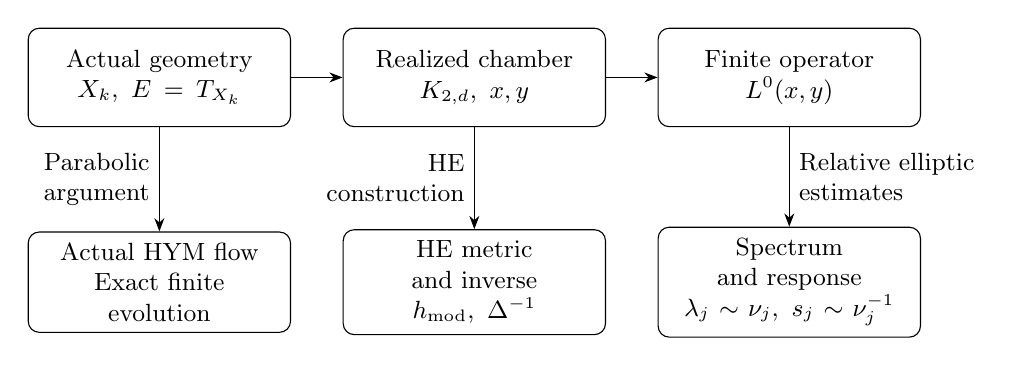
\begin{tikzpicture}[>=Stealth, every node/.style={font=\small},
 block/.style={draw,rounded corners,align=center,text width=3.05cm,
 minimum height=1.25cm,inner sep=4pt}]
\node[block] (geometry) at (0,0) {Actual geometry\\\(X_k,\ E=T_{X_k}\)};
\node[block] (chamber) at (4,0) {Realized chamber\\\(K_{2,d},\ x,y\)};
\node[block] (finite) at (8,0) {Finite operator\\\(L^0(x,y)\)};
\node[block] (flow) at (0,-2.6) {Actual HYM flow\\Exact finite evolution};
\node[block] (metric) at (4,-2.6) {HE metric and inverse\\\(h_{\rm mod},\ \Delta^{-1}\)};
\node[block] (spectrum) at (8,-2.6) {Spectrum and response\\\(\lambda_j\sim\nu_j,\ s_j\sim\nu_j^{-1}\)};
\draw[->] (geometry)--(chamber);
\draw[->] (chamber)--(finite);
\draw[->] (geometry)--node[left,align=right] {Parabolic\\argument} (flow);
\draw[->] (chamber)--node[left,align=right] {HE\\construction} (metric);
\draw[->] (finite)--node[right,align=left] {Relative elliptic\\estimates} (spectrum);
\end{tikzpicture}
\caption{The common family in Theorem~\ref{thm01:synthesis}.
All statements concern the same tangent extension. The finite
operator includes harmonic extension data; the flow requires
its separate parabolic argument. The lower assertions do not
follow from the chamber alone.}
\label{fig01:synthesis}
\end{figure}


\subsection*{Proof strategy and relation to prior work}
The response proof begins with compact-unitary equivariance of the
elliptic complementary solution. Differentiating it controls
commutators relative to the energy of each weak graph direction.
At actual HE, adjunction preserves the real operator; its Schur
form is consequently a relative perturbation of the graph form.
Denote this Schur operator by \(S\). Let \(T\) be the block-scalar
projection of the intrinsic metric velocity generated by a
variation of the diagonal balancing potential.
Exact differentiation factors the reduced Jacobian as \(MST\).
The metric velocity contains the same \(T\), which cancels before
the singular inverse is applied. The remaining background derivative
is bounded, whereas every inverse graph singular value diverges;
this proves all response singular values with coefficient one.

For several-factor flows the noncommuting exponential velocity is
retained in the slice equation. Its exact principal-part cancellation
gives a common-domain parabolic system. A finite-regularity invariant
manifold, with its full correction, reconstructs exact flows.
Bipartite mass coercivity confines their total conductance for all
future time without requiring each edge to decrease. Qualitative
reference matching and fixed-time parameter comparison supply a
restart; order preservation then has zero future residual. This
explains the quantifier order \(\varepsilon\), then \(T\), then
\(U_\varepsilon\). The signed two-factor theorem in
Section~\ref{sec05:signed} instead uses a radial integrable-error
family and a calibrated scalar clock. Its unstable tail requires
separation of variables rather than a fixed speed perturbation.

Local HYM wall-crossing and quantitative continuity are established
prior work, notably Clarke--Tipler \cite{clarketipler2024} and
Delloque \cite{delloque2025}; the latter already gives a quantitative
connection estimate and treats nonabelian deformation theory.
Sektnan--Tipler \cite{sektnantipler2024} provides a related
adiabatic analytic framework. Earlier two-factor endomorphism
spectra and flow matching are developed in
\cite{wuebben2026walls,wuebben2026flow}. Our claims concern the
specified intrinsic derivative and inverse spectrum at all positive
ratios, the signed joint profile, and exact corrected all-future
comparison in the stated two-step class, rather than the first
quantitative continuity statement.

Finite reductions and iterated-logarithmic metric growth also have
substantial predecessors. Haiden--Katzarkov--Kontsevich--Pandit
develop the finite theory in \cite{hkkp2023}, and the metric order
and approximate-flow comparisons in \cite[\S4.2]{hkkp2018}; their
geometric metric-growth theorem there is for curves. Lam
\cite{lam2026} treats semistable bundles with locally free graded
object and bounded iterated-logarithmic remainder. Those bounded
remainders are not asserted to converge. Our nearby-parameter
relative small-spectrum theorem retains an exact corrected finite
field instead of inferring near-one comparison from a bounded
metric sandwich. The domain-valued parabolic graph uses Simonett's
parameter theorem \cite{simonett1994} with the explicit hypotheses
checked in Section~\ref{sec06:graph}.

% ============================================================
% section_02_stationary.tex
% ============================================================
\section{The common stationary model}\label{sec02:stationary}

Let \(X\) be a compact connected Kähler manifold of complex
dimension \(n\), and let
\(\omega_s\) be a smooth finite-dimensional family of Kähler forms
near \(s=0\). Fix the holomorphic extension
\begin{equation}\label{eq02:extension}
 0\longrightarrow S:=\bigoplus_{i\in I}F_i
 \longrightarrow E\longrightarrow U:=\bigoplus_{j\in J}F_j
 \longrightarrow0.
\end{equation}
The \(m\) factors are pairwise nonisomorphic, locally free and stable
with equal slope at \(\omega_0\). There is one edge \(e:j\to i\)
for each nonzero component of the fixed extension class. Assume this
bipartite support is connected. Multiple basis vectors in one Ext
space are part of that single component, not additional edges.

Write \(r_v=\rk F_v\), \(M=\diag(r_v)\), \(R=\sum_vr_v\),
and let the incidence column be \(D_e=e_i-e_j\). Continue normalized
factor HE metrics \(h_{v,s}\) smoothly and represent the fixed
classes by harmonic \(\beta_{e,s}\). These are the usual local
factor continuation and harmonic projection constructions; for the
line factors in our geometric application they also follow directly
from the scalar Poisson equation. Set
\begin{equation}\label{eq02:normalization}
 \begin{aligned}
 V_s&=\int_X\omega_s^n/n!,&
 \kappa_v&=\frac{2\pi}{(n-1)!V_sr_v}
                  c_1(F_v)[\omega_s]^{n-1},\\
 \kappa_E&=R^{-1}\sum_vr_v\kappa_v,&
 b_v&=-r_v(\kappa_v-\kappa_E),&
 c_e(s)&=V_s^{-1}\|\beta_{e,s}\|_{L^2}^2>0.
 \end{aligned}
\end{equation}
The demand vector \(b\) has ordinary sum zero. This name refers
only to the displayed centered slope vector. Potentials, in contrast,
will be rank-centered: \(\sum_vr_vx_v=0\).

On the fixed smooth direct sum put
\begin{equation}\label{eq02:amplitude}
 \db_{s,t}=\db_0+N_{s,t},\qquad
 N_{s,t}=\sum_et_e\beta_{e,s},\qquad h_{0,s}=\bigoplus_vh_{v,s}.
\end{equation}
Every amplitude assignment is integrable, including complex or zero
amplitudes, because \(N\) maps \(U\) to \(S\) and vanishes on
\(S\). A positive diagonal gauge \(g_x=\diag(e^{x_v/2})\) sends
the amplitude-one bundle to the amplitudes
\(t_e=e^{(D^Tx)_e/2}\). With cycles, arbitrary independent amplitudes
need not belong to this fixed orbit.

The amplitude-one presentation is identified with the original
\(E\) by a smooth time-independent triangular map \(\Phi_s\).
Indeed \(\beta_s-\beta_{\rm ref}=\db a_s\), with \(a_s:U\to S\)
chosen smoothly by the split Green operator. The relevant degree-zero
cross-Hom kernels vanish at the wall and nearby. Since products of
two such blocks vanish, \(\Phi_s=I\pm a_s\) is an exact isomorphism
with determinant one. We keep this identification in every metric
formula on \(E\).

We normalize the reference splitting so that \(\beta_{\rm ref}\)
has zero block on every pair \((i,j)\) whose extension class vanishes.
Such a block is \(\db\)-exact and is removed by a triangular
change of splitting. Blockwise harmonic projection and the split
Green operator then keep these blocks zero for every \(s\).
Thus \(a_s\), and hence \(\Phi_s-I\), are supported only on
edges of the fixed graph. This convention is used in
Lemma~\ref{lem04:background}.

Let
\begin{equation}\label{eq02:scalarspace}
 \HH=\{X=\diag(X_vI_{F_v}):X_v\in\RR,\ \sum_vr_vX_v=0\},
 \qquad \langle X,Y\rangle_M=\sum_vr_vX_vY_v.
\end{equation}
This is the real parallel trace-free scalar space. On real Hermitian
pointwise trace-free sections use the normalized inner product
\(V_s^{-1}\int_X\tr(AB)\,dV_s\), which induces exactly this mass
inner product on \(\HH\). Write \(P_s\) for its orthogonal
projection and \(Q_s=1-P_s\). Smooth block-diagonal isometries fix
all scalar sections and identify these spaces uniformly as \(s\)
varies. All spatial estimates below use these identifications.

For a metric \(h\), write \(K_h=i\Lambda_{\omega_s}F_h\).
The centered curvature is
\[
 \cK(s,t,u)=e^{u/2}K_{\db_{s,t},h_{0,s}e^u}e^{-u/2}-\kappa_EI,
 \qquad P_su=0,
\]
where \(u\) is Hermitian and pointwise trace free. The determinant
metric is unchanged and has constant curvature trace, so
\(\tr\cK=0\) pointwise. At the split metric the real linearization is
\begin{equation}\label{eq02:realoperator}
 L_s=\tfrac12(\Delta_{\db,s}+\Delta_{\partial,s}).
\end{equation}
The Chern metric-variation identities are those of
\cite[\S4.2, equations~(4.2.12)--(4.2.16)]{kobayashi1987}.
Its wall kernel is exactly \(\HH\); the stable distinct factors
exclude cross-Hom sections. Its normal restriction has a uniform
elliptic gap. The implicit-function theorem therefore solves
\(Q_s\cK=0\) uniquely for a small smooth \(u=u(s,t)\), with
\begin{equation}\label{eq02:complement}
 \|u(s,t)\|_{C^a}\le C_a|t|^2,\qquad
 \|D_tu(s,t)\|_{C^a}\le C_a|t|
\end{equation}
for each fixed spatial order. Harmonicity removes the first amplitude
derivative for every nearby \(s\). This construction, including
complex amplitudes as real parameters, is the elliptic complementary
construction used below. It differs from the parabolic invariant
manifold of Section~\ref{sec06:graph}.

We state precisely the independent stationary input from
\cite[Theorem~1.1]{wuebben2026uniform}.

\begin{theorem}[Stationary two-step comparison]\label{thm02:stationary}
Locally \(E\) is stable exactly when \(b\in D\RR_{>0}^{E(\Gamma)}\).
For such \(b\) the unique rank-centered balancing potential \(x^0\)
satisfies
\begin{equation}\label{eq02:balance}
 k_e=c_e(s)e^{(D^Tx^0)_e},\qquad Dk=b,
 \qquad\sigma=\sum_ek_e=\sum_{i\in I}b_i.
\end{equation}
An actual HE metric is obtained with \(x=x^0+y\),
\(\|y\|_\infty\le C\sigma\), and the complementary solution
\(u(s,t)\), where \(t_e=e^{(D^Tx)_e/2}\).
Its determinant-normalized fixed-bundle metric satisfies
\begin{equation}\label{eq02:metric}
 e^{-C\sigma}\Phi_s^*\!\left(\bigoplus_ve^{x_v^0}h_{v,s}\right)
 \le H_s\le
 e^{C\sigma}\Phi_s^*\!\left(\bigoplus_ve^{x_v^0}h_{v,s}\right).
\end{equation}
If \(\nu_1(k)\le\cdots\le\nu_{m-1}(k)\) are the positive
eigenvalues of \(M^{-1/2}D\diag(k)D^TM^{-1/2}\), the complex
trace-free endomorphism Dolbeault spectrum has
\begin{equation}\label{eq02:spectrum}
 \lambda_j=\nu_j(k)(1+O(\sigma))\quad(j<m),\qquad
 \lambda_m\ge\gamma>0.
\end{equation}
All errors remain uniform as any positive normalized cut capacity
or ratio of positive graph eigenvalues tends to zero. No fixed
positive lower bound for these quantities is required.
\end{theorem}

The mechanism of the input is relevant to the new estimates. Exponential
balancing minimizes the strictly convex coercive function
\(\sum_ec_e e^{(D^Tx)_e}-b\cdot x\) on rank-centered potentials.
The reduced curvature equation is
\(-b+D(c_et_e^2)+\mathcal R=0\), with amplitude jets through order
three vanishing in \(\mathcal R\), parameterwise. For every cut
\(C\), the exact splitting trace identity gives
\[
 |\mathcal R_C|\le C|t|^2\sum_{e\in\partial C}t_e^2.
\]
The weighted graph inverse controls oscillation by
\( (m-1)\max_C |q_C|/\sum_{e\in\partial C}k_e\).
It yields \(y=O(\sigma)\) without a bound on the ordinary graph
inverse. For the spectrum, harmonicity gives
\(\db_0^*[N_{s,t},X]=0\) on block scalars; the resulting
complementary coupling is small relative to their graph energy.
Schur elimination and min--max then compare every ordered mode,
including repetitions. These are the cut and spectral arguments of
\cite[\S\S3--5]{wuebben2026uniform}, not a parameter-derivative
conclusion from \eqref{eq02:metric}.

Constants throughout this paper concern fixed factors, support,
nonzero extension classes and a controlled smooth background family.
They are not uniform if classes vanish or the number of factors grows.

\begin{lemma}\label{lem02:amplitudespectrum}
Let all amplitudes be positive and small, without requiring balance.
For any metric \(h_0e^v\) with \(\|v\|_{C^0}\le C|t|^2\),
the complex \(\End_0\) Dolbeault eigenvalues satisfy
\[
 \lambda_j=\nu_j(c_et_e^2)(1+O(|t|^2))\quad(j<m),\qquad
 \lambda_m\ge\gamma>0.
\]
This is a complex spectral statement and requires no HE equation.
\end{lemma}

\begin{proof}
First use the split metric and decompose into the complex block-scalar
kernel and its orthogonal complement. The scalar energy is exactly
\(q_t(X)=\sum_ec_et_e^2|(D^TX)_e|^2\). Harmonic cancellation
gives the off-diagonal block bound
\(\|B_tX\|^2\le C|t|^2q_t(X)\), and the complementary form
has a fixed gap. At a spectral parameter \(0\le\mu\le C|t|^2\),
Schur elimination subtracts
\(B_t^*(C_t-\mu)^{-1}B_t\), a nonnegative form at most
\(C|t|^2q_t\). Inertia, or equivalently the min--max principle
for this Schur family, places each ordered small eigenvalue between
\((1-C|t|^2)\nu_j\) and \(\nu_j\). The rank of the scalar
space is \(m-1\), while the complement keeps its gap.
Finally \(e^v\) changes degree-zero and degree-one endomorphism
norms multiplicatively by \(e^{O(|t|^2)}\). Rayleigh quotients
transfer the same relative comparison to the asserted metric.
\end{proof}

% ============================================================
% section_03_inverse.tex
% ============================================================
\section{The real HE operator and its inverse}\label{sec03:inverse}

Fix an actual HE zero from Theorem~\ref{thm02:stationary}, at its
corrected amplitudes \(t\). Suppress \(s\), and put
\begin{equation}\label{eq03:energy}
 \widetilde k_e=c_e(s)t_e^2,\qquad
 q(X)=\sum_e\widetilde k_e|(D^TX)_e|^2,
 \qquad \mathcal L=M^{-1}D\diag(\widetilde k)D^T\big|_{\HH}.
\end{equation}
Thus \(q=\langle X,\mathcal LX\rangle_M\),
\(|t|^2\asymp\sigma\), \(q(X)\le C\sigma\|X\|_M^2\), and
\(q=(1+O(\sigma))q_k\) as quadratic forms.
No lower bound for this energy on a unit vector is used.

Use the unitary identification
\(\mathscr U(Y)=e^{u/2}Ye^{-u/2}\) from the metric \(h_0e^u\)
to \(h_0\). The HE Dolbeault Laplacian becomes a self-adjoint
operator \(\Delta\) in this fixed realization. It preserves the
real Hermitian subspace: adjunction exchanges \(\Delta_{\db}\) and
\(\Delta_\partial\), while their difference on endomorphism
zero-forms is the curvature commutator, which vanishes at HE.
This use of the HE equation is essential for the real block argument.

\begin{lemma}\label{lem03:phase}
For every fixed spatial order \(a\),
\begin{equation}\label{eq03:phase}
 \|[u,X]\|_{C^a}+\|u_x[X]\|_{C^a}
       \le C_a\sqrt\sigma\sqrt{q(X)},\qquad X\in\HH,
\end{equation}
where \(u_x[X]=D_tu[(t_e(D^TX)_e/2)_e]\).
\end{lemma}

\begin{proof}
The complementary solution exists smoothly for complex amplitudes
\(z\) and obeys \(\|D_zu\|_{C^a}\le C_a|z|\).
For \(U_\theta=e^{i\theta X}\), uniqueness gives
\[
 u\bigl(s,(e^{i\theta(D^TX)_e}z_e)_e\bigr)
       =U_\theta u(s,z)U_\theta^{-1}.
\]
Differentiating at \(\theta=0\) gives
\[
 i[X,u]=D_zu\bigl[(i(D^TX)_ez_e)_e\bigr].
\]
At the real amplitudes \(z=t\),
\[
 \|D_zu\|_{\RR^{2|E(\Gamma)|}\to C^a}
       \le C_a|t|\le C_a\sqrt\sigma,\qquad
 \sum_et_e^2|(D^TX)_e|^2\le c_{\min}^{-1}q(X).
\]
These bounds prove the commutator estimate. The ordinary chain rule
with amplitude velocity \(t_e(D^TX)_e/2\) gives the same bound
for \(u_x[X]\).
\end{proof}

For later use define the analytic even operators
\begin{equation}\label{eq03:exponential}
 C_u=\cosh(\ad_u/2),\qquad
 S_u=\frac{\sinh(\ad_u/2)}{\ad_u/2},\qquad
 Z_u=\sinh(\ad_u/2),
\end{equation}
with their continuous values at zero. Two commutators and
\(u=O(\sigma)\) imply
\begin{equation}\label{eq03:evenbounds}
 \|Z_uX\|_{C^a}\le C_a\sqrt\sigma\sqrt{q(X)},\qquad
 \|(C_u-I)X\|_{C^a}\le C_a\sigma^{3/2}\sqrt{q(X)}.
\end{equation}

\begin{proposition}\label{prop03:schur}
In the orthogonal decomposition \(\HH\oplus Q\), write
\begin{equation}\label{eq03:blocks}
 \Delta=\begin{pmatrix}G&B^*\\ B&C\end{pmatrix}.
\end{equation}
The complement has \(C\ge\gamma I\), and
\begin{equation}\label{eq03:blockbounds}
 \begin{aligned}
 |\langle X,GX\rangle_M-q(X)|&\le C_0\sigma q(X),\\
 \|BX\|_{L^2/V}^2&\le C_0\sigma q(X),\\
 S:=G-B^*C^{-1}B&=(1+O(\sigma))\mathcal L
                       \quad\hbox{as quadratic forms on }\HH.
 \end{aligned}
\end{equation}
\end{proposition}

\begin{proof}
For a physical block scalar \(X\), harmonicity gives
\(\db_0^*[N,X]=0\). Hence, in the split metric,
\[
 \|\Delta_{h_0,t}X\|_{L^2/V}
 =\|[N,\cdot]^*[N,X]\|_{L^2/V}
 \le C\sqrt\sigma\sqrt{q(X)}.
\]
Changing the inner products in degrees zero and one by \(e^u\)
changes the first-order formal adjoint by coefficients \(O(\sigma)\)
in each required spatial norm. This follows by conjugating the split
adjoint by the positive Gram matrices. Applied to \(\db_tX\),
it adds at most \(C\sigma\sqrt{q(X)}\). In the centered realization
the vector \(X\) corresponds to \(e^{-u/2}Xe^{u/2}\).
Lemma~\ref{lem03:phase} bounds the difference in \(C^2\) by
\(C\sqrt\sigma\sqrt{q(X)}\); the operator has uniformly bounded
second-order coefficients there. Projection proves the bound on \(B\).

The physical scalar energy is \(q(X)(1+O(\sigma))\), by multiplicative
metric comparison. Its centered image is \(C_uX+Z_uX\), with
Hermitian and skew-Hermitian parts. Since \(\Delta\) preserves
adjunction at HE, their real energies add orthogonally.
Equation~\eqref{eq03:evenbounds} gives energy at most
\(C\sigma q(X)\) for \(Z_uX\) and at most \(C\sigma^3q(X)\)
for \((C_u-I)X\). The energy triangle inequality and then
Cauchy--Schwarz show that the energy of the centered \(X\) is
\(q(X)(1+O(\sigma))\). This is the asserted bound on \(G\).

The split complement has a uniform gap. Smooth coefficients, elliptic
estimates and compactness preserve it on \(Q\) for the nearby
centered operator. The bounded inverse \(C^{-1}\) and the bound on
\(B\) give
\(0\le B^*C^{-1}B\le(C_0/\gamma)\sigma\mathcal L\).
Subtracting proves the relative Schur-form estimate.
\end{proof}

The complement is defined by its closed form on \(QH^1\), with
operator domain \(QH^2\). Here and below the projections act on
the real Hermitian pointwise trace-free section bundle. They are
uniformly smooth finite-rank modifications of the identity, so the
usual elliptic domain and regularity statements persist.

\begin{theorem}\label{thm03:inverse}
Let \(J:\HH\to\HH\oplus Q\) be \(JX=X-C^{-1}BX\). Then
\begin{equation}\label{eq03:inverse}
 Q\Delta J=0,\qquad J^*\Delta J=S,\qquad
 \Delta^{-1}=JS^{-1}J^*+QC^{-1}Q.
\end{equation}
Moreover
\begin{equation}\label{eq03:lift}
 \|JX-X\|_{L^2/V}\le C\sqrt\sigma\sqrt{q(X)},\qquad
 J^*J=I+O(\sigma^2),
\end{equation}
and for each fixed nonnegative integer \(a\),
\begin{equation}\label{eq03:sobolev}
 \|C^{-1}v\|_{H^{a+2}}\le C_a\|v\|_{H^a},\qquad
 \|(J-I)X\|_{H^{a+2}}\le C_a\sqrt\sigma\sqrt{q(X)}.
\end{equation}
The inverse norm is \(\nu_1(k)^{-1}(1+O(\sigma))\).
For every real \(z\ge0\), set
\[
 C_z=C+zI,\quad J_zX=X-C_z^{-1}BX,
 \quad S_z=G+zI-B^*C_z^{-1}B.
\]
Then the exact positive-resolvent formula and form estimates are
\begin{equation}\label{eq03:resolvent}
 \begin{gathered}
 (\Delta+zI)^{-1}=J_zS_z^{-1}J_z^*+QC_z^{-1}Q,\\
 (1-C_1\sigma)q(X)+z\|X\|_M^2
 \le\langle X,S_zX\rangle_M
 \le(1+C_1\sigma)q(X)+z\|X\|_M^2,\\
 \|J_zX-X\|_{L^2/V}
 \le\frac{\sqrt{C_0}\sqrt\sigma}{\gamma+z}\sqrt{q(X)}.
 \end{gathered}
\end{equation}
Here \(C_1=C_0(1+\gamma^{-1})\).
\end{theorem}

\begin{proof}
Solving the complementary block gives \(Qv=C^{-1}(Qf-BPv)\).
Substitution into the scalar block gives \(SPv=J^*f\).
Proposition~\ref{prop03:schur} proves \(S>0\), so this elimination
is legitimate and proves \eqref{eq03:inverse}. The estimates on \(B\)
give \eqref{eq03:lift}; in particular
\(J^*J-I=B^*C^{-2}B=O(\sigma^2)\) because
\(q(X)\le C\sigma\|X\|_M^2\). Uniform elliptic estimates with the
gap controlling the \(L^2\) term give \eqref{eq03:sobolev}; use
the same smooth harmonic cancellation at the required spatial order
for \(BX\). The complex spectrum in \eqref{eq02:spectrum} agrees
with the real Hermitian spectrum at HE, giving the inverse norm.

The identical elimination with \(C+zI\) proves the resolvent identity.
Its correction is nonnegative and bounded by
\(C_0\sigma q/(\gamma+z)\),
uniformly for \(z\ge0\), proving its form estimates. Finally
\(\|C_z^{-1}\|\le(\gamma+z)^{-1}\) gives the last bound.
\end{proof}

These identities give a linear HE metric-equation inverse with its
possibly large finite response separated from a uniformly regular
complement. They are not a nonlinear gauge choice on a quotient
moduli space. The spatial norms are in the scaled harmonic
presentation and the unitary identification above; they are not
uniform bounds in an arbitrary unbounded fixed-bundle frame.
Only real nonnegative spectral shifts are asserted.

% ============================================================
% section_04_response.tex
% ============================================================
\section{Every intrinsic metric-response singular value}\label{sec04:response}

Assume the slope map \(s\mapsto b(s)\) has rank \(m-1\) at
the reference point. Work in a smooth parameter chart \(s=s(b,\zeta)\)
with bounded derivatives near the wall, holding \(\zeta\) fixed.
On inputs use the dual mass norm
\begin{equation}\label{eq04:input}
 \|\dot b\|_{M^{-1}}^2=\sum_v\dot b_v^2/r_v,
 \qquad f=M^{-1}\dot b\in\HH.
\end{equation}
On outputs use the real Hermitian normalized \(L^2\) norm at the
actual metric \(H_s\). Define the intrinsic logarithmic tangent
\begin{equation}\label{eq04:response}
 \mathscr D_s\dot b=(H_s^{-1}\partial_{\dot b}H_s)_0,
\end{equation}
where the subscript is pointwise trace-free projection. It is
\(H_s\)-Hermitian. This is the intrinsic tangent to the space of
positive Hermitian forms, not \(d(\log H_s)\) in a fixed matrix
frame. Smooth scalar normalizations of \(H_s\) do not affect it.

Let \(F(s,x)\) be the mass-weighted reduced curvature vector: at a
complementary solution its component is
\(r_v(P_s\cK)_v\). At an HE zero use the operators of
Section~\ref{sec03:inverse} and put
\begin{equation}\label{eq04:velocity}
 V_X=C_uX+S_uu_x[X],\qquad TX=PV_X.
\end{equation}

\begin{lemma}\label{lem04:differentiate}
At every constructed HE zero,
\begin{equation}\label{eq04:factorization}
 Q\Delta V_X=0,\qquad V_X=JTX,\qquad
 T=I+O(\sigma^2),\qquad F_x=MST.
\end{equation}
\end{lemma}

\begin{proof}
Differentiate the metric
\(g_x^*(h_0e^{u(s,t(x))})\) in the direction \(X\), then transport
to the centered unitary realization. Since \(g_x=e^{x/2}\), its
two diagonal-gauge terms sum to \(C_uX\), and the exponential
derivative gives \(S_uu_x[X]\). Thus its centered velocity is
exactly \eqref{eq04:velocity}, with coefficient one.
For a varying conjugation \(a\), its derivative contributes
\([\dot a a^{-1},aKa^{-1}]\). Applied successively to \(g_x\)
and \(e^{u/2}\), both terms vanish at the scalar HE curvature.
Here the second logarithmic derivative is
\((\partial_Xe^{u/2})e^{-u/2}\); no commutation of \(u\) and
\(u_x[X]\) is required. Also \(\Delta_\partial=\Delta_{\db}\)
at HE. Differentiating \(Q\cK=0\) therefore gives
\(Q\Delta V_X=0\). Complementary elimination gives \(V_X=JPV_X\).
Since \(Pu_x=0\), \(C_u-I,S_u-I=O(u^2)\), and
\(u_x[X]=O(\sigma)\|X\|_M\), projection gives
\(T=I+O(\sigma^2)\). Finally differentiating \(F=MP\cK\)
at the zero gives \(F_x=MP\Delta V=MST\).
\end{proof}

This also proves smooth dependence inside the stable chamber.
Both \(S\) and \(T\) are invertible, so the ordinary finite
implicit-function theorem gives a smooth root near each HE zero.
The determinant-normalized HE metric on the simple stable \(E\)
is unique. Hence these local metric branches agree. Their coordinates
agree as well. Fix an interior parameter \(s_0\). For \(s\)
sufficiently close to \(s_0\), continuity of \(x^0(s)\) on the
open chamber places the branches, relative to
\(g_{x^0(s_0)}\), in one small slice chart
\((y,u)\mapsto e^{y/2}e^ue^{y/2}\), whose derivative at zero is
an isomorphism from \(\HH\oplus Q\). This neighborhood may
depend on \(s_0\). The branches patch without
differentiating a choice in the stationary Brouwer construction.
No smooth extension of the diverging \(x\) to the boundary is asserted.

\begin{lemma}\label{lem04:background}
At fixed \(x\), the reduced curvature derivative and full metric
derivative satisfy
\begin{equation}\label{eq04:background}
 F_b\dot b=-\dot b+E_1\dot b,
 \qquad \|M^{-1}E_1\dot b\|_M\le C\sigma\|\dot b\|_{M^{-1}},
 \qquad \|H_b\dot b\|_{L^2/V}\le C\|\dot b\|_{M^{-1}}.
\end{equation}
Here \(H_b\) denotes the intrinsic trace-free fixed-\(x\) metric
derivative, in the centered realization.
\end{lemma}

\begin{proof}
The reduced equation is \(-b+D(c_et_e^2)+\mathcal R\).
Smooth harmonic coefficients with bounded derivatives give
\(D(c_{e,b}t_e^2)=O(\sigma)\|\dot b\|\).
The amplitude jets of \(\mathcal R\) through order three vanish
for every background parameter. Taylor's formula therefore bounds
its first background derivative by \(C|t|^4\|\dot b\|\).
The derivative of \(-b\) is exactly \(-\dot b\), proving the
first assertion. It is an ordinary forcing bound, not a cut-relative
estimate; the exact inverse will be retained.

For the metric derivative one must account for the possibly
unbounded \(g_x\). In the triangular harmonic identification,
\(\Phi_b\Phi_s^{-1}=\pm a_b\) is still a sum of \(U\to S\)
blocks. Products of two such blocks vanish. Therefore
\begin{equation}\label{eq04:triangular}
 (g_x\Phi_b\Phi_s^{-1}g_x^{-1})_e=\pm t_ea_{e,b},\qquad
 \|g_x\Phi_b\Phi_s^{-1}g_x^{-1}\|_{C^a}
       \le C_a\sqrt\sigma\|\dot b\|.
\end{equation}
By the reference-splitting normalization in
Section~\ref{sec02:stationary}, \(a_b\) has no block on a pair
without an edge, so no unscaled block appears.
The background metric derivative is block
diagonal and commutes with \(g_x\). The derivative \(u_b\) at
fixed \(t\) is \(O(\sigma)\). Smooth centered exponential
identities, these bounds, and the bounded parameter chart prove
the assertion about \(H_b\). Varying unitary background frames
adds bounded terms; curvature conjugation derivatives vanish at HE.
\end{proof}

\begin{theorem}\label{thm04:response}
Let \(s_1(\mathscr D_s)\ge\cdots\ge s_{m-1}(\mathscr D_s)\)
be the singular values from \eqref{eq04:input} to the normalized
real Hermitian \(L^2\) output norm. For every sufficiently small
stable parameter,
\begin{equation}\label{eq04:singular}
 s_j(\mathscr D_s)=\frac{1+O(\sigma)}{\nu_j(k(s,b))},
 \qquad 1\le j<m.
\end{equation}
The error remains uniform as positive normalized cut capacities
or ratios of positive graph eigenvalues tend to zero, also when
eigenvalues repeat. It uses the current harmonic coefficients.
\end{theorem}

\begin{proof}
Differentiate \(F(s(b),x(b))=0\). The two lemmas give
\(ST\dot x=(I+E)f\), with \(\|E\|_{M\to M}\le C\sigma\).
The full centered intrinsic velocity is \(JT\dot x+H_b\dot b\),
so the exact cancellation is
\begin{equation}\label{eq04:exactresponse}
 \mathscr D_s\dot b=JS^{-1}(I+E)f+H_b\dot b.
\end{equation}
In particular, no ordinary error in \(T\) is multiplied through an
ill-conditioned inverse.

Relative Schur-form comparison and min--max bracket each eigenvalue
of \(S\) by \((1+O(\sigma))\nu_j(k)\). Thus each decreasing
singular value of \(S^{-1}\) is
\((1+O(\sigma))/\nu_j(k)\). Right multiplication by \(I+E\)
changes every singular value by \(1+O(\sigma)\), and left
multiplication by \(J\) changes it by \(1+O(\sigma^2)\), since
\(J^*J=I+O(\sigma^2)\). These are singular-value min--max
inequalities and require no commutation. Finally the trace identity gives
\[
 \sum_{j=1}^{m-1}\nu_j(k)
 =\sum_{e:j\to i}k_e(r_i^{-1}+r_j^{-1})\le2\sigma,
\]
so \(\nu_{m-1}\le2\sigma\). Hence even the smallest singular value
of this principal response is at least \(c/\sigma\).
The additive perturbation bound
\(|s_j(A+H)-s_j(A)|\le\|H\|\), with the bounded \(H_b\),
changes every value only relatively by \(O(\sigma)\).
The input map \(\dot b\mapsto M^{-1}\dot b\) is an isometry
in the stated norms, proving the theorem with coefficient one.
\end{proof}

For two factors with conductance \(\beta>0\), the positive graph
eigenvalue is \(\beta(r_1+r_2)/(r_1r_2)\). The rank-centered
metric potential difference is \(\log(\beta/c)\). Its output norm
divided by the dual-mass input norm is
\(r_1r_2/((r_1+r_2)\beta)\), checking the coefficient in
\eqref{eq04:singular}.

The theorem is not a directional relative expansion by the graph
inverse: noncommuting form perturbations can rotate widely separated
eigenspaces. It asserts the exact decomposition
\eqref{eq04:exactresponse}, the relative Schur form, and all singular
values. If the slope map realizes only a proper subspace of the
centered slope directions, the response is restricted to that
subspace; its singular values need not recover the entire
graph spectrum. Replacing current \(c(s)\) by \(c(0)\) gives error
\(O(\sigma+|s|)\) unless \(|s|=O(\sigma)\) is separately proved.

% ============================================================
% section_05_signed.tex
% ============================================================
\section{The signed two-factor transition}\label{sec05:signed}

There is a closed joint profile for two factors. Its proof uses the
elliptic complementary family and an integrable future error. The
several-factor theorem will instead use the exact parabolic graph.
The distinction matters on the unstable side, where a fixed error
in an exponential rate would destroy all-future relative control.

We use the following order principle in both arguments. Its
arbitrary-dimensional form is the metric comparison of
\cite[Propositions~4.3 and 4.5]{hkkp2018}.

\begin{lemma}\label{lem05:order}
Let \(h\) be an exact normalized HYM flow, and let a positive metric
family \(H\) on the same holomorphic bundle and base form have full
logarithmic residual
\[
 \mathcal E_H=H^{-1}\dot H+2(K_H-\kappa_EI),\qquad
 \|\mathcal E_H\|_{\infty,\mathrm{op},H}\le f(\tau).
\]
If \(e^{-\eta}aH(T)\le h(T)\le e^\eta aH(T)\), then for every
future time of existence
\begin{equation}\label{eq05:barrier}
 e^{-\eta-\int_T^\tau f}aH(\tau)
 \le h(\tau)\le
 e^{\eta+\int_T^\tau f}aH(\tau).
\end{equation}
For exact \(H\), the integral is zero. A sandwich
\(e^{-\eta}aH\le h\le e^\eta aH\) changes every \(\End_0\)
Dolbeault eigenvalue by factors between \(e^{-4\eta}\) and
\(e^{4\eta}\).
\end{lemma}

\begin{proof}
Multiplying the approximate family by
\(\exp(\pm\int_T^\tau f)\) adds respectively \(\pm fI\) to
its logarithmic velocity and changes no curvature, since the scalar
is spatially constant. Its residual is therefore nonnegative or
nonpositive as a Hermitian endomorphism. The tensor maximum
principle for HYM metric order, applied at the first contact of
the largest relative eigenvalue, gives the two barriers. This
uses the displayed full residual, so no half-gauge-velocity
normalization is suppressed. On endomorphisms a metric sandwich
changes squared norms in degrees zero and one by \(e^{\pm2\eta}\).
The scalar \(a\) cancels, and min--max gives the spectral factors.
\end{proof}

Now let \(0\to F\to E\to G\to0\) be nonsplit, with distinct
stable locally free factors of equal slope at \(s=0\). Put
\(a=\rk F\), \(b=\rk G\), \(R=a+b\), and
\begin{equation}\label{eq05:radialdata}
 q=\diag((b/R)I_F,-(a/R)I_G),\qquad
 \delta_s=\kappa_G(s)-\kappa_F(s),\qquad
 c_s=\frac{\|\beta_s\|^2}{V_sab/R}.
\end{equation}
The complementary curvature is exactly
\(\cK(s,t,u(s,t))=k_s(t)q\), where
\(k_s(t)=-\delta_s+c_st^2+O(t^4)\). Conjugation by
\(\diag(-I_F,I_G)\) makes this scalar even in \(t\), although
the whole correction \(u\) need not be even. Thus
\begin{equation}\label{eq05:calibrated}
 z_s(w)=k_s(\sqrt w)+\delta_s=c_sw+O(w^2),\qquad
 z_s'(w)=c_s+O(w)>0
\end{equation}
is smooth up to \(w=0\), jointly in \(s\). Only this scalar is
asserted smooth in \(w\).

Choose \(w(T)=w_0\) above the positive equilibrium if
\(\delta_s>0\), and solve
\begin{equation}\label{eq05:radial}
 \dot w=-2w(z_s(w)-\delta_s),\qquad t=\sqrt w,
 \qquad H_s^{[T]}=\Phi_s^*(t^q)^*(h_{0,s}e^{u(s,t)}).
\end{equation}
The solution is positive at finite times, monotone, and tends to
\(w_\dagger\), where \(z_s(w_\dagger)=\delta_s\) for
\(\delta_s>0\) and \(w_\dagger=0\) otherwise.
Lemma~\ref{lem02:amplitudespectrum} gives
\(\lambda_1(H_s^{[T]})/z_s(w)=1+O(w)\) and a fixed next gap.

\begin{lemma}\label{lem05:residual}
The metric in \eqref{eq05:radial} has full residual bounded by
\(Cw|z_s(w)-\delta_s|\), and
\begin{equation}\label{eq05:integrable}
 \int_T^\infty\|\mathcal E_{H_s^{[T]}}\|_{\infty,\mathrm{op}}
 \,d\tau\le C(w_0-w_\dagger)\le Cw_0.
\end{equation}
\end{lemma}

\begin{proof}
Write \(k=k_s(t)\). The diagonal gauge velocity is \(-kq\).
After transport by \(t^q\), the residual is exactly
\[
 -k\bigl(e^{-u}qe^u+q-2e^{-u/2}qe^{u/2}\bigr)
                  +e^{-u}\partial_\tau e^u.
\]
The parenthesis is \((\mathcal A_u-I)^2q\), where
\(\mathcal A_uX=e^{-u/2}Xe^{u/2}\), so it is \(O(w^2)\).
The exponential derivative formula and
\(\|u_t\|\le C|t|\), \(\dot t=-tk\), bound the second term
by \(Cw|k|\). Transported and intrinsic norms differ by a bounded
factor \(e^{O(w)}\), irrespective of the diagonal gauge size.
Finally \(w|z_s(w)-\delta_s|=|\dot w|/2\); monotonicity proves
the integrable estimate. The residual vanishes at equilibrium.
\end{proof}

Define the positive signed profile
\begin{equation}\label{eq05:profile}
 P_\delta(\tau)=
 \begin{cases}\displaystyle\frac{\delta}{1-e^{-2\delta\tau}},
       &\delta\ne0,\\[5pt]
 \displaystyle\frac1{2\tau},&\delta=0.
 \end{cases}
\end{equation}

\begin{lemma}\label{lem05:scalar}
Suppose \(w_0\to0\) and \(2Tz_0(w_0)\to1\) along a reference
restart sequence \(T\to\infty\). For every \(\varepsilon>0\),
one sufficiently late \(T\) and one neighborhood \(U\) give
\[
 \sup_{s\in U,\ \tau\ge T}
 \left|\frac{z_s(w_s^{[T]}(\tau))}{P_{\delta_s}(\tau)}-1\right|
 <\varepsilon.
\]
Both signs of \(\delta_s\) and all sizes of \(\delta_s\tau\)
are included.
\end{lemma}

\begin{proof}
Writing \(z=z_s(w)\), its exact equation is
\(\dot z=-2\alpha_s(z)z(z-\delta_s)\), where
\(\alpha_s=wz_s'/z_s=1+O(w)=1+O(z)\), uniformly.
For \(\delta\ge0\), compare with the constant-speed solutions
\[
 Y_r(\tau)=\frac{\delta}
 {1-(1-\delta/z_0)e^{-2r\delta(\tau-T)}}
 \quad(\delta>0),\qquad
 Y_r(\tau)=\frac{z_0}{1+2rz_0(\tau-T)}\quad(\delta=0),
\]
using \(r=1\pm Cw_0\). Put
\(\eta=|2Tz_0-1|+|r-1|+2\delta T\). For small \(\eta\),
we have \(\delta<z_0\), so the trajectory starts above equilibrium.
The offset
\(\theta=-T-\log(1-\delta/z_0)/(2r\delta)\), with its
continuous zero-gap value, has \(|\theta|/T\le C\eta\).
The ratio to \(P_\delta\) is
\((1-e^{-x})/(1-e^{-r(1+\theta/\tau)x})\), \(x=2\delta\tau\).
Monotonicity and concavity of \(1-e^{-x}\) bound this ratio by
\(1+O(\eta)\), uniformly for every \(x\ge0\).

For \(\delta=-d<0\), constant speed perturbations would change
the exponential rate. Instead put
\(Q=\log(1+d/z)\), \(Q_0=\log(1+d/z_0)\), and
\(L=2d(\tau-T)\). Then \(Q=Q_0+L+E\), with
\(E=2d\int_T^\tau(\alpha_s(z)-1)\,dv\).
The pointwise estimate gives \(|E|\le Cz_0L\). Separation of
variables, using \(\alpha_s\ge1/2\), also gives
\[
 |E|\le Cd\log\frac{z_0+d}{z(\tau)+d}\le Cz_0.
\]
Thus \(|E|\le Cz_0\min(Q_0+L,1)\). For small \(z_0\) this
is at most \((Q_0+L)/2\), so every intermediate argument in the
following mean-value estimate is at least \((Q_0+L)/2\). Since
\((\log(e^x-1))'\le1+1/x\), the solution differs from its
unit-speed \(Y_1\) by logarithmic relative error \(O(z_0)\)
for the entire future interval. For that unit-speed solution the
offset is \(\theta=-T+\log(1+d/z_0)/(2d)\).
If \(\eta=|2Tz_0-1|+2dT\) is small, then
\(|\theta|/T\le C\eta\); applying the same logarithmic derivative
bound to exponents \(2d\tau\) and \(2d(\tau+\theta)\) gives
logarithmic relative error \(O(\eta)\) to \(P_{-d}\), even at
exponentially late times.

Choose \(T\) first so that the reference clock and \(w_0\) errors
are small. For that fixed \(T\), continuity of \(z_s(w_0)\)
and \(\delta_s\to0\) gives a neighborhood where
\(|2Tz_s(w_0)-1|\), \(|\delta_s|T\), and \(z_s(w_0)\)
are small. Positive-gap trajectories start above equilibrium.
The two estimates prove the assertion, with no comparison of
\(|s|\) to the possibly much smaller \(|\delta_s|\).
\end{proof}

\begin{theorem}\label{thm05:joint}
For any smooth positive initial-metric family on the fixed two-factor
extension, let \(h_s(\tau)\) solve normalized HYM flow. For every
\(\varepsilon>0\) there are a finite \(T\) and a neighborhood
\(U\) of zero such that for all \(s\in U\) and \(\tau\ge T\),
\begin{equation}\label{eq05:joint}
 \left|\frac{\lambda_1(h_s(\tau),\omega_s)}
                         {P_{\delta_s}(\tau)}-1\right|<\varepsilon.
\end{equation}
There are also one fixed late time, neighborhood and positive lower
bound for \(\lambda_2\) throughout their future interval.
\end{theorem}

\begin{proof}
The qualitative matching lemma proved in Section~\ref{sec08:matching}
uses only reference convergence and the two-step holomorphic
filtration. It gives \(T\to\infty\), \(w_T\to0\), scalars
\(a_T>0\), and \(\eta_T\to0\) with
\(h_0(T)\in e^{\pm\eta_T}a_TH_0(w_T)\).
We first calibrate the clock without assuming a joint theorem.
At the wall the radial solution has \(\dot z=-2(1+o(1))z^2\),
so \(\tau z\to1/2\) for any fixed restart. Lemmas
\ref{lem05:order}--\ref{lem05:residual} compare the exact reference
trajectory with it at all future times with logarithmic error
\(\eta_T+Cw_T\). Letting these restart errors tend to zero proves
\(2\tau\lambda_1(h_0(\tau))\to1\). Evaluating at \(T\), and
using the matching and model spectral estimate, gives
\(2Tz_0(w_T)\to1\).

For each fixed late \(T\), finite-time parameter continuity gives
\(h_s(T)\in e^{\pm o_T(1)}h_0(T)\) and
\(H_s(w_T)\in e^{\pm o_T(1)}H_0(w_T)\). One direct proof of
the first assertion regards \(h_0\) on \([0,T]\) as an
approximate \(\omega_s\)-flow: its residual is
\(2i(\Lambda_{\omega_s}-\Lambda_{\omega_0})F_{h_0}
 -2(\kappa_E(s)-\kappa_E(0))I=O_T(|s|)\), and the initial
metrics are close. Apply Lemma~\ref{lem05:order}.
After choosing \(T\), shrink the neighborhood so that these
restart errors and \(|\delta_s|T\) are small. The residual integral
is \(O(w_T)\) uniformly for all future times. The scalar lemma,
model spectral estimate and metric Rayleigh comparison prove
\eqref{eq05:joint}. One fixed sufficiently late restart supplies
the complementary gap as well.
\end{proof}

For \(\delta>0\) the profile tends to \(\delta\); at the wall
it is \(1/(2\tau)\); for \(\delta<0\) it is asymptotic to
\(|\delta|e^{-2|\delta|\tau}\). The theorem includes all these
regimes and their joint transitions. Its spectrum is that of the
endomorphism Dolbeault Laplacian; it does not identify the full
Yang--Mills Hessian or a nonlinear contraction rate.

% Native figure source: figures/code/fig05_profile.tex
\begin{figure}[htbp]
\centering
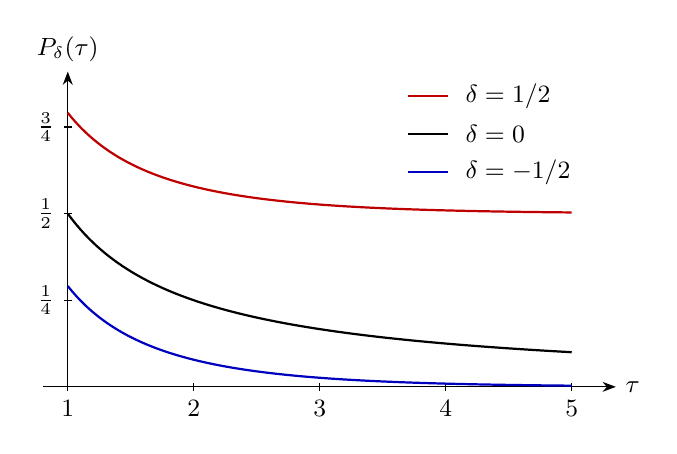
\begin{tikzpicture}[x=1.6cm,y=4.4cm,>=Stealth,every node/.style={font=\small}]
\draw[->] (.8,0)--(5.35,0) node[right] {\(\tau\)};
\draw[->] (1,0)--(1,.91) node[above] {\(P_\delta(\tau)\)};
\draw (1,.012)--(1,-.012) node[below] {1};
\draw (2,.012)--(2,-.012) node[below] {2};
\draw (3,.012)--(3,-.012) node[below] {3};
\draw (4,.012)--(4,-.012) node[below] {4};
\draw (5,.012)--(5,-.012) node[below] {5};
\draw (.97,0.25)--(1.03,0.25);\node[left] at (.97,0.25) {$\tfrac14$};
\draw (.97,0.5)--(1.03,0.5);\node[left] at (.97,0.5) {$\tfrac12$};
\draw (.97,0.75)--(1.03,0.75);\node[left] at (.97,0.75) {$\tfrac34$};
\draw[thick,red!75!black] plot coordinates {(1.0000000000,0.7909883534) (1.0333333333,0.7761792676) (1.0666666667,0.7623738462) (1.1000000000,0.7494803295) (1.1333333333,0.7374177414) (1.1666666667,0.7261143493) (1.2000000000,0.7155063803) (1.2333333333,0.7055369464) (1.2666666667,0.6961551385) (1.3000000000,0.6873152603) (1.3333333333,0.6789761771) (1.3666666667,0.6711007601) (1.4000000000,0.6636554090) (1.4333333333,0.6566096428) (1.4666666667,0.6499357454) (1.5000000000,0.6436084584) (1.5333333333,0.6376047147) (1.5666666667,0.6319034052) (1.6000000000,0.6264851755) (1.6333333333,0.6213322469) (1.6666666667,0.6164282590) (1.7000000000,0.6117581313) (1.7333333333,0.6073079398) (1.7666666667,0.6030648087) (1.8000000000,0.5990168133) (1.8333333333,0.5951528935) (1.8666666667,0.5914627775) (1.9000000000,0.5879369121) (1.9333333333,0.5845664018) (1.9666666667,0.5813429523) (2.0000000000,0.5782588214) (2.0333333333,0.5753067735) (2.0666666667,0.5724800392) (2.1000000000,0.5697722781) (2.1333333333,0.5671775459) (2.1666666667,0.5646902638) (2.2000000000,0.5623051911) (2.2333333333,0.5600174001) (2.2666666667,0.5578222530) (2.3000000000,0.5557153816) (2.3333333333,0.5536926676) (2.3666666667,0.5517502254) (2.4000000000,0.5498843860) (2.4333333333,0.5480916826) (2.4666666667,0.5463688365) (2.5000000000,0.5447127449) (2.5333333333,0.5431204698) (2.5666666667,0.5415892268) (2.6000000000,0.5401163759) (2.6333333333,0.5386994119) (2.6666666667,0.5373359567) (2.7000000000,0.5360237510) (2.7333333333,0.5347606474) (2.7666666667,0.5335446037) (2.8000000000,0.5323736766) (2.8333333333,0.5312460162) (2.8666666667,0.5301598605) (2.9000000000,0.5291135302) (2.9333333333,0.5281054244) (2.9666666667,0.5271340162) (3.0000000000,0.5261978482) (3.0333333333,0.5252955296) (3.0666666667,0.5244257317) (3.1000000000,0.5235871851) (3.1333333333,0.5227786766) (3.1666666667,0.5219990461) (3.2000000000,0.5212471840) (3.2333333333,0.5205220286) (3.2666666667,0.5198225636) (3.3000000000,0.5191478158) (3.3333333333,0.5184968533) (3.3666666667,0.5178687831) (3.4000000000,0.5172627494) (3.4333333333,0.5166779317) (3.4666666667,0.5161135433) (3.5000000000,0.5155688296) (3.5333333333,0.5150430665) (3.5666666667,0.5145355591) (3.6000000000,0.5140456404) (3.6333333333,0.5135726699) (3.6666666667,0.5131160325) (3.7000000000,0.5126751373) (3.7333333333,0.5122494166) (3.7666666667,0.5118383248) (3.8000000000,0.5114413375) (3.8333333333,0.5110579503) (3.8666666667,0.5106876785) (3.9000000000,0.5103300558) (3.9333333333,0.5099846335) (3.9666666667,0.5096509801) (4.0000000000,0.5093286802) (4.0333333333,0.5090173341) (4.0666666667,0.5087165571) (4.1000000000,0.5084259787) (4.1333333333,0.5081452422) (4.1666666667,0.5078740042) (4.2000000000,0.5076119337) (4.2333333333,0.5073587122) (4.2666666667,0.5071140324) (4.3000000000,0.5068775986) (4.3333333333,0.5066491257) (4.3666666667,0.5064283389) (4.4000000000,0.5062149733) (4.4333333333,0.5060087736) (4.4666666667,0.5058094938) (4.5000000000,0.5056168964) (4.5333333333,0.5054307525) (4.5666666667,0.5052508415) (4.6000000000,0.5050769505) (4.6333333333,0.5049088742) (4.6666666667,0.5047464145) (4.7000000000,0.5045893802) (4.7333333333,0.5044375871) (4.7666666667,0.5042908572) (4.8000000000,0.5041490189) (4.8333333333,0.5040119065) (4.8666666667,0.5038793601) (4.9000000000,0.5037512253) (4.9333333333,0.5036273534) (4.9666666667,0.5035076003) (5.0000000000,0.5033918275)};
\draw[thick,black] plot coordinates {(1.0000000000,0.5000000000) (1.0333333333,0.4838709677) (1.0666666667,0.4687500000) (1.1000000000,0.4545454545) (1.1333333333,0.4411764706) (1.1666666667,0.4285714286) (1.2000000000,0.4166666667) (1.2333333333,0.4054054054) (1.2666666667,0.3947368421) (1.3000000000,0.3846153846) (1.3333333333,0.3750000000) (1.3666666667,0.3658536585) (1.4000000000,0.3571428571) (1.4333333333,0.3488372093) (1.4666666667,0.3409090909) (1.5000000000,0.3333333333) (1.5333333333,0.3260869565) (1.5666666667,0.3191489362) (1.6000000000,0.3125000000) (1.6333333333,0.3061224490) (1.6666666667,0.3000000000) (1.7000000000,0.2941176471) (1.7333333333,0.2884615385) (1.7666666667,0.2830188679) (1.8000000000,0.2777777778) (1.8333333333,0.2727272727) (1.8666666667,0.2678571429) (1.9000000000,0.2631578947) (1.9333333333,0.2586206897) (1.9666666667,0.2542372881) (2.0000000000,0.2500000000) (2.0333333333,0.2459016393) (2.0666666667,0.2419354839) (2.1000000000,0.2380952381) (2.1333333333,0.2343750000) (2.1666666667,0.2307692308) (2.2000000000,0.2272727273) (2.2333333333,0.2238805970) (2.2666666667,0.2205882353) (2.3000000000,0.2173913043) (2.3333333333,0.2142857143) (2.3666666667,0.2112676056) (2.4000000000,0.2083333333) (2.4333333333,0.2054794521) (2.4666666667,0.2027027027) (2.5000000000,0.2000000000) (2.5333333333,0.1973684211) (2.5666666667,0.1948051948) (2.6000000000,0.1923076923) (2.6333333333,0.1898734177) (2.6666666667,0.1875000000) (2.7000000000,0.1851851852) (2.7333333333,0.1829268293) (2.7666666667,0.1807228916) (2.8000000000,0.1785714286) (2.8333333333,0.1764705882) (2.8666666667,0.1744186047) (2.9000000000,0.1724137931) (2.9333333333,0.1704545455) (2.9666666667,0.1685393258) (3.0000000000,0.1666666667) (3.0333333333,0.1648351648) (3.0666666667,0.1630434783) (3.1000000000,0.1612903226) (3.1333333333,0.1595744681) (3.1666666667,0.1578947368) (3.2000000000,0.1562500000) (3.2333333333,0.1546391753) (3.2666666667,0.1530612245) (3.3000000000,0.1515151515) (3.3333333333,0.1500000000) (3.3666666667,0.1485148515) (3.4000000000,0.1470588235) (3.4333333333,0.1456310680) (3.4666666667,0.1442307692) (3.5000000000,0.1428571429) (3.5333333333,0.1415094340) (3.5666666667,0.1401869159) (3.6000000000,0.1388888889) (3.6333333333,0.1376146789) (3.6666666667,0.1363636364) (3.7000000000,0.1351351351) (3.7333333333,0.1339285714) (3.7666666667,0.1327433628) (3.8000000000,0.1315789474) (3.8333333333,0.1304347826) (3.8666666667,0.1293103448) (3.9000000000,0.1282051282) (3.9333333333,0.1271186441) (3.9666666667,0.1260504202) (4.0000000000,0.1250000000) (4.0333333333,0.1239669421) (4.0666666667,0.1229508197) (4.1000000000,0.1219512195) (4.1333333333,0.1209677419) (4.1666666667,0.1200000000) (4.2000000000,0.1190476190) (4.2333333333,0.1181102362) (4.2666666667,0.1171875000) (4.3000000000,0.1162790698) (4.3333333333,0.1153846154) (4.3666666667,0.1145038168) (4.4000000000,0.1136363636) (4.4333333333,0.1127819549) (4.4666666667,0.1119402985) (4.5000000000,0.1111111111) (4.5333333333,0.1102941176) (4.5666666667,0.1094890511) (4.6000000000,0.1086956522) (4.6333333333,0.1079136691) (4.6666666667,0.1071428571) (4.7000000000,0.1063829787) (4.7333333333,0.1056338028) (4.7666666667,0.1048951049) (4.8000000000,0.1041666667) (4.8333333333,0.1034482759) (4.8666666667,0.1027397260) (4.9000000000,0.1020408163) (4.9333333333,0.1013513514) (4.9666666667,0.1006711409) (5.0000000000,0.1000000000)};
\draw[thick,blue!75!black] plot coordinates {(1.0000000000,0.2909883534) (1.0333333333,0.2761792676) (1.0666666667,0.2623738462) (1.1000000000,0.2494803295) (1.1333333333,0.2374177414) (1.1666666667,0.2261143493) (1.2000000000,0.2155063803) (1.2333333333,0.2055369464) (1.2666666667,0.1961551385) (1.3000000000,0.1873152603) (1.3333333333,0.1789761771) (1.3666666667,0.1711007601) (1.4000000000,0.1636554090) (1.4333333333,0.1566096428) (1.4666666667,0.1499357454) (1.5000000000,0.1436084584) (1.5333333333,0.1376047147) (1.5666666667,0.1319034052) (1.6000000000,0.1264851755) (1.6333333333,0.1213322469) (1.6666666667,0.1164282590) (1.7000000000,0.1117581313) (1.7333333333,0.1073079398) (1.7666666667,0.1030648087) (1.8000000000,0.0990168133) (1.8333333333,0.0951528935) (1.8666666667,0.0914627775) (1.9000000000,0.0879369121) (1.9333333333,0.0845664018) (1.9666666667,0.0813429523) (2.0000000000,0.0782588214) (2.0333333333,0.0753067735) (2.0666666667,0.0724800392) (2.1000000000,0.0697722781) (2.1333333333,0.0671775459) (2.1666666667,0.0646902638) (2.2000000000,0.0623051911) (2.2333333333,0.0600174001) (2.2666666667,0.0578222530) (2.3000000000,0.0557153816) (2.3333333333,0.0536926676) (2.3666666667,0.0517502254) (2.4000000000,0.0498843860) (2.4333333333,0.0480916826) (2.4666666667,0.0463688365) (2.5000000000,0.0447127449) (2.5333333333,0.0431204698) (2.5666666667,0.0415892268) (2.6000000000,0.0401163759) (2.6333333333,0.0386994119) (2.6666666667,0.0373359567) (2.7000000000,0.0360237510) (2.7333333333,0.0347606474) (2.7666666667,0.0335446037) (2.8000000000,0.0323736766) (2.8333333333,0.0312460162) (2.8666666667,0.0301598605) (2.9000000000,0.0291135302) (2.9333333333,0.0281054244) (2.9666666667,0.0271340162) (3.0000000000,0.0261978482) (3.0333333333,0.0252955296) (3.0666666667,0.0244257317) (3.1000000000,0.0235871851) (3.1333333333,0.0227786766) (3.1666666667,0.0219990461) (3.2000000000,0.0212471840) (3.2333333333,0.0205220286) (3.2666666667,0.0198225636) (3.3000000000,0.0191478158) (3.3333333333,0.0184968533) (3.3666666667,0.0178687831) (3.4000000000,0.0172627494) (3.4333333333,0.0166779317) (3.4666666667,0.0161135433) (3.5000000000,0.0155688296) (3.5333333333,0.0150430665) (3.5666666667,0.0145355591) (3.6000000000,0.0140456404) (3.6333333333,0.0135726699) (3.6666666667,0.0131160325) (3.7000000000,0.0126751373) (3.7333333333,0.0122494166) (3.7666666667,0.0118383248) (3.8000000000,0.0114413375) (3.8333333333,0.0110579503) (3.8666666667,0.0106876785) (3.9000000000,0.0103300558) (3.9333333333,0.0099846335) (3.9666666667,0.0096509801) (4.0000000000,0.0093286802) (4.0333333333,0.0090173341) (4.0666666667,0.0087165571) (4.1000000000,0.0084259787) (4.1333333333,0.0081452422) (4.1666666667,0.0078740042) (4.2000000000,0.0076119337) (4.2333333333,0.0073587122) (4.2666666667,0.0071140324) (4.3000000000,0.0068775986) (4.3333333333,0.0066491257) (4.3666666667,0.0064283389) (4.4000000000,0.0062149733) (4.4333333333,0.0060087736) (4.4666666667,0.0058094938) (4.5000000000,0.0056168964) (4.5333333333,0.0054307525) (4.5666666667,0.0052508415) (4.6000000000,0.0050769505) (4.6333333333,0.0049088742) (4.6666666667,0.0047464145) (4.7000000000,0.0045893802) (4.7333333333,0.0044375871) (4.7666666667,0.0042908572) (4.8000000000,0.0041490189) (4.8333333333,0.0040119065) (4.8666666667,0.0038793601) (4.9000000000,0.0037512253) (4.9333333333,0.0036273534) (4.9666666667,0.0035076003) (5.0000000000,0.0033918275)};
\draw[thick,red!75!black] (3.7,0.84)--(4.02,0.84);\node[right] at (4.08,0.84) {$\delta=1/2$};
\draw[thick,black] (3.7,0.73)--(4.02,0.73);\node[right] at (4.08,0.73) {$\delta=0$};
\draw[thick,blue!75!black] (3.7,0.62)--(4.02,0.62);\node[right] at (4.08,0.62) {$\delta=-1/2$};
\end{tikzpicture}
\caption{The proved two-factor profile on the stable side, at the wall, and on the unstable side. These are evaluations of formula~\eqref{eq05:profile}, not measured HYM trajectories. Uniform relative comparison in Theorem~\ref{thm05:joint} includes the entire future interval after its late restart.}
\label{fig05:profile}
\end{figure}


% ============================================================
% section_06_graph.tex
% ============================================================
\section{An exact finite evolution for the flow}\label{sec06:graph}

The elliptic complementary metrics do not in general form an invariant
manifold for HYM flow. We construct a separate parabolic graph and
retain its exact finite field. Each Kähler parameter \(s\) remains
constant along a trajectory.

For a general small normal \(u\), retain \(\cK(s,t,u)\) from
Section~\ref{sec02:stationary} and \(C_u,S_u\) from
\eqref{eq03:exponential}. Set
\begin{equation}\label{eq06:finiteoperator}
 B_u=S_u^{-1}C_u,\qquad \mathcal R_s(u)=P_sB_u|_{\HH}.
\end{equation}
In an eigenbasis of \(u\), \(S_u\) has eigenvalue
\(\sinh a/a>0\), and \(B_u\) has eigenvalue \(a\coth a>0\),
where \(a=(u_i-u_j)/2\). They preserve real Hermitian sections
and trace. The finite operator \(\mathcal R_s(u)\) is positive
and invertible, with \(\mathcal R_s(u)=I+O(\|u\|_\infty^2)\).
Define
\begin{equation}\label{eq06:slice}
 \begin{aligned}
 A(s,t,u)&=-\mathcal R_s(u)^{-1}P_sS_u^{-1}\cK(s,t,u),\\
 \dot t_e&=(A_i-A_j)t_e,\qquad (e:j\to i),\\
 \dot u&=-2S_u^{-1}\cK(s,t,u)-2B_uA(s,t,u).
 \end{aligned}
\end{equation}
Here \(A\in\HH\), so its components are rank-centered.

\begin{proposition}\label{prop06:exact}
System~\eqref{eq06:slice} preserves \(P_su=0\) and pointwise trace
zero. Every classical solution reconstructs an exact normalized HYM
flow on the bundle at its initial amplitudes. It preserves every zero
edge, every nonzero amplitude sign, and its initial diagonal orbit.
\end{proposition}

\begin{proof}
Integrate \(\dot gg^{-1}=A\), starting from a positive diagonal
gauge. Its determinant stays one. The amplitude equation gives
\(N_{t(\tau)}=g(\tau)N_{t(T)}g(\tau)^{-1}\), with the initial
gauge included in this identity as appropriate. On that fixed bundle
the reconstructed metric is \(H=g^*(h_{0,s}e^u)\). Centering its
velocity gives exactly
\begin{equation}\label{eq06:velocity}
 2C_uA+S_u\dot u=-2\cK.
\end{equation}
Indeed the two gauge terms are
\(e^{-u/2}Ae^{u/2}+e^{u/2}Ae^{-u/2}\), and
\[
 e^{-u/2}(\partial_\tau e^u)e^{-u/2}
   =\int_{-1/2}^{1/2}e^{\theta\ad_u}\dot u\,d\theta=S_u\dot u.
\]
Solving \eqref{eq06:velocity} subject to \(P_s\dot u=0\) gives
exactly \eqref{eq06:slice}. Its pointwise trace is zero because
\(\tr\cK=\tr A=0\) and the commutator functions preserve trace.
The multiplicative amplitude equations preserve signs and zeroes.
For \(h\in\ker D\), they give
\(\partial_\tau\sum_eh_e\log|t_e|=h^TD^TA=0\) on nonzero
support. Thus the evolution stays on its initial diagonal orbit.
\end{proof}

\subsection{The normal equation and its domain}

The highest-derivative coefficient in centered Chern curvature is
the same \(S_u\) as in the velocity. At a contracted second jet
\(W\) the metric-change formula gives
\[
 e^{-u/2}(d\exp)_u(W)e^{-u/2}=S_uW.
\]
All derivatives of this coefficient and all extension terms use
only first spatial jets. Consequently there is an exact identity
\begin{equation}\label{eq06:principal}
 S_u^{-1}\cK=L_su+K_{{\rm split},s}
                  +\mathcal G_s(t,u,\nabla_su),\qquad
 K_{{\rm split},s}=\diag(-b_v/r_v),
\end{equation}
where \(\mathcal G_s\) depends only on the first jet and its value
and first derivatives vanish at \((t,u)=(0,0)\). The amplitude
derivative vanishes by current harmonicity; the normal derivative
is the definition of the full real split linearization.
Self-adjointness and \(L_s\HH=0\) imply \(P_sL_su=0\), so
\eqref{eq06:slice} takes the form
\begin{equation}\label{eq06:semilinear}
 \begin{aligned}
 A&=-\mathcal R_s(u)^{-1}(K_{{\rm split},s}+P_s\mathcal G_s),\\
 \dot u&=-2L_su+\mathcal N_s(t,u),\\
 \mathcal N_s&=-2\mathcal G_s
 +2(B_u\mathcal R_s(u)^{-1}-I)K_{{\rm split},s}
 +2B_u\mathcal R_s(u)^{-1}P_s\mathcal G_s.
 \end{aligned}
\end{equation}
Both first derivatives of \(\mathcal N_s\) vanish at the origin,
for every nearby \(s\). In particular no extra \(b_su\) normal
linear term remains. The edge linearization there is
\begin{equation}\label{eq06:edgelinear}
 (\Lambda_s)_{ee}=b_i/r_i-b_j/r_j\longrightarrow0.
\end{equation}

We verify a concrete continuous-maximal-regularity realization of
Simonett's parameter theorem \cite[Theorem~2.1]{simonett1994}.
Let \(h^q\) denote little-Hölder sections, the closure of smooth
sections in the nonintegral Hölder norm, of the real Hermitian
pointwise trace-free bundle \(\mathcal V_s\). Smooth block
isometries identify it with \(\mathcal V_0\). The maps
\(T_s=Q_s|_{Q_0}\) and their inverses identify all normal spaces
uniformly. Put \(u=T_sv\) and take
\begin{equation}\label{eq06:spaces}
 \begin{aligned}
 X_0&=\RR^{E(\Gamma)}\oplus Q_0h^{3/8}(\mathcal V_0),&
 X_1&=\RR^{E(\Gamma)}\oplus Q_0h^{19/8}(\mathcal V_0),\\
 X_\beta&=(X_0,X_1)^0_{5/8,\infty}
       =\RR^{E(\Gamma)}\oplus Q_0h^{13/8},&
 X_\alpha&=(X_0,X_1)^0_{7/8,\infty}
       =\RR^{E(\Gamma)}\oplus Q_0h^{17/8}.
 \end{aligned}
\end{equation}
The superscript zero denotes continuous real interpolation. All
spatial exponents are nonintegral. The bounded finite-rank projection
preserves these interpolation identities. A first derivative of
\(u\in h^{13/8}\) lies in \(h^{5/8}\subset h^{3/8}\).
Hölder multiplication, smooth matrix functions near zero and the
finite inverse in \eqref{eq06:semilinear} therefore make every
nonlinear term a smooth map from a neighborhood in \(X_\beta\)
to \(X_0\), jointly with \(s\).

The principal operator is the smooth common-domain family
\(\mathcal A(s)=\diag(0,2T_s^{-1}L_sT_s):X_1\to X_0\).
It has continuous maximal regularity on this scale. One can apply
the normally elliptic little-Hölder theorem
\cite[Remark~3.3 and Proposition~3.7]{shaosimonett2014} to the
endomorphism bundle as follows. Embed the real bundle into a
trivial bundle with an orthogonal complement, extend \(L_s\) by
a connection Laplacian on that complement with the same scalar
principal symbol, and apply the local matrix-valued elliptic
resolvent proof on the trivial bundle. Restriction to the reducing
original summand gives the bundle result. Since \(P_s\) commutes
with \(L_s\), uniqueness of the linear parabolic solution restricts
maximal regularity to \(Q_s\) with its full domain. Conjugation
by \(T_s\) and the finite-dimensional zero summand preserve it.
The estimates are locally uniform in \(s\).

At the wall the flow linearization is
\(\diag(0,-2L_0|_{Q_0})\), with finite center and uniformly negative
normal spectrum. Thus all hypotheses of the parameter-dependent
invariant-manifold theorem hold. Keeping \(L_s\) in its
common-domain operator family is necessary: treating
\((L_s-L_0)u\) as a lower-order term on \(X_\beta\) would lose
two derivatives.

\begin{theorem}\label{thm06:graph}
Fix a finite integer \(\ell\ge4\). On a sufficiently small common
parameter/amplitude neighborhood there is a jointly \(C^\ell\) map
\(\Psi(s,t)\in Q_sh^{19/8}(\mathcal V_s)\) whose graph is locally
invariant for \eqref{eq06:slice}, contains every equilibrium
sufficiently small in the domain norm of \(X_1\) and inside the
construction's cutoff neighborhood, and satisfies
\begin{equation}\label{eq06:graphbound}
 \Psi(s,0)=0,\quad D_t\Psi(s,0)=0,\quad
 \|\Psi(s,t)\|_{C^2}\le C|t|^2,\quad
 \|D_t\Psi(s,t)\|_{C^2}\le C|t|.
\end{equation}
It may be chosen equivariant under constant vertex signs. Substitution
\(u=\Psi(s,t)\) in \eqref{eq06:slice}, with its exact \(A\),
defines one finite corrected field. Its trajectories reconstruct
exact classical HYM solutions while they remain in the domain.
\end{theorem}

\begin{proof}
The preceding verification and \cite[Theorem~2.1]{simonett1994}
give a graph valued in the full normal domain \(h^{19/8}\), not
merely in the interpolation space. Every \((s,0,0)\) is an
equilibrium, so it lies on the graph. Differentiate the invariance
identity at \(t=0\). If \(H_s=D_t(T_s^{-1}\Psi)(s,0)\), then
\(H_s\Lambda_s=B_sH_s\), where
\(B_s=-2T_s^{-1}L_sT_s\). Shrink so each eigenvalue of
\(\Lambda_s\) has absolute value below the fixed normal gap.
Each \(B_s-(\Lambda_s)_{ee}\) is invertible, whence \(H_s=0\).
Taylor's formula, jointly in \(s\) and \(t\), gives the uniform
quadratic bounds at every nearby split equilibrium.

For vertex signs \(\varepsilon_v\), conjugation by
\(U_\varepsilon=\diag(\varepsilon_vI)\) sends
\(t_e\) to \(\varepsilon_i\varepsilon_jt_e\) and \(u\) to
\(U_\varepsilon uU_\varepsilon^{-1}\). It preserves the exact
equations and all projections. In the fixed-point construction of
the invariant manifold choose invariant norms and a radial smooth
cutoff in the finite amplitude space. The transformed graph solves
the same integral fixed-point equation and belongs to the same
uniqueness class. Hence that constructed graph is equivariant.
This uses no averaging of graphs and no smooth Banach-space norm.

Local invariance and parabolic uniqueness identify a reduced
trajectory with \eqref{eq06:slice}. Since the graph is \(C^1\)
into the full \(h^{19/8}\) domain, its reconstructed metric is
\(C^1\) in time with continuous second spatial derivatives, and
the parabolic equation holds pointwise. Proposition~\ref{prop06:exact}
then gives an exact classical HYM solution.
\end{proof}

\enlargethispage{-2\baselineskip}
The graph is a chosen finite-regularity object and is not canonical.
The construction can be made at any prescribed finite spatial order
by shifting all exponents in \eqref{eq06:spaces}. We neither identify
graphs obtained on different scales nor assert a single infinitely
differentiable graph. Equilibria on disconnected supports need not
be HE metrics; the equilibrium-inclusion statement alone says no more.

% ============================================================
% section_07_confinement.tex
% ============================================================
\section{Confinement without a lower cut bound}\label{sec07:confinement}

Fix the invariant graph of Theorem~\ref{thm06:graph}. On it write
\begin{equation}\label{eq07:field}
 A=M^{-1}(b-p)+E_s(t),\qquad
 k_e=c_e(s)t_e^2,\quad p=Dk,\quad\sigma=\sum_ek_e.
\end{equation}
The quadratic projected curvature term is \(M^{-1}Dk\).
The projected split linearization annihilates the normal variable
exactly; substituting \(\Psi=O(|t|^2)\) in the smooth equations
therefore gives
\begin{equation}\label{eq07:error}
 \|E_s(t)\|_M\le C|t|^3\le K\sigma^{3/2}.
\end{equation}
In particular there is no suppressed \(|b||t|^2\) term.
The contributions of the split scalar curvature through
\(\mathcal R_s(u)^{-1}-I\) and \(S_u^{-1}-I\) are
\(O(|b||t|^4)\), since both operators differ from the identity
by \(O(u^2)\). They are absorbed in \(C|t|^3\) on the fixed
bounded parameter neighborhood. The proof
will only use this cubic bound, not a higher-order sign improvement.

Let \(R_I=\sum_{i\in I}r_i\), \(R_J=\sum_{j\in J}r_j\), and put
\[
 \rho_*=R_I^{-1}+R_J^{-1},\qquad
 C_*^2=(\min_{i\in I}r_i)^{-1}+(\min_{j\in J}r_j)^{-1}.
\]
Since all arrows go from \(J\) to \(I\),
\begin{equation}\label{eq07:mass}
 \sum_{i\in I}p_i=\sigma,\quad\sum_{j\in J}p_j=-\sigma,
 \qquad \rho_*\sigma^2\le\|p\|_{M^{-1}}^2\le C_*^2\sigma^2.
\end{equation}
The lower estimate is weighted Cauchy--Schwarz on each part. For
the upper estimate, the components have one sign on each part,
so the sum of their squares is at most the square of their sum.
This estimate allows every nonnegative conductance ratio.

\begin{proposition}\label{prop07:confinement}
There is a fixed small threshold \(\sigma_*\) such that, if at a
restart \(T\) the amplitudes are positive,
\begin{equation}\label{eq07:initial}
 0<\sigma(T)=\sigma_0<\sigma_*,\qquad
 \|b\|_{M^{-1}}\le\frac{\rho_*}{4C_*}\sigma_0,
\end{equation}
the exact finite trajectory exists for every \(\tau\ge T\), stays
in the graph domain, and satisfies \(0<\sigma(\tau)\le\sigma_0\).
At \(b=0\),
\begin{equation}\label{eq07:wallbound}
 \sigma(\tau)\le\frac{\sigma_0}{1+\rho_*\sigma_0(\tau-T)}.
\end{equation}
\end{proposition}

\begin{proof}
Since \(s\) is fixed, the amplitude equations give exactly
\[
 \dot\sigma=2p\cdot A
  =-2\|p\|_{M^{-1}}^2+2p^TM^{-1}b+2p\cdot E_s(t).
\]
Using \eqref{eq07:error}--\eqref{eq07:mass} and shrinking the
threshold to absorb \(2C_*K\sigma^{5/2}\), we obtain
\begin{equation}\label{eq07:logisticbound}
 \dot\sigma\le-\rho_*\sigma^2+2C_*\|b\|_{M^{-1}}\sigma.
\end{equation}
At a first upward crossing of \(\sigma_0\) this derivative would
be at most \(-\rho_*\sigma_0^2/2\), a contradiction. Choosing
\(\sigma_*\) smaller if necessary keeps
\(|t|^2\le\sigma_0/c_{\min}\) inside a strictly smaller amplitude
ball, and the quadratic graph bound keeps the normal variable
inside its domain. Finite-dimensional continuation gives the
all-future solution. Positivity persists at every finite time by
the multiplicative equations. At \(b=0\), integrate
\(\dot\sigma\le-\rho_*\sigma^2\) to obtain
\eqref{eq07:wallbound}.
\end{proof}

No individual edge must decrease. For unit masses, targets \(1,2\),
sources \(3,4\), take leading conductances
\[
 (k_{13},k_{14},k_{23},k_{24})
     =(\epsilon,\epsilon^2,\epsilon^2,1),\qquad
 b=(2\epsilon,\epsilon,-2\epsilon,-\epsilon).
\]
For the leading field the first edge grows because
\(A_1-A_3=2\epsilon-2\epsilon^2>0\), while
\(A_2-A_4=-2+2\epsilon-2\epsilon^2<0\). Scaling both the
conductances and \(b\) by a common small positive number places
the example in an arbitrarily small amplitude neighborhood; for
sufficiently small \(\epsilon\), \eqref{eq07:initial} holds and
the total decreases. This explains why the scalar total, rather
than separate edge monotonicity, is the appropriate confinement
quantity. The exact corrected field, rather than its leading term,
is used in the proposition and all subsequent comparisons.

% ============================================================
% section_08_matching.tex
% ============================================================
\section{Matching prescribed actual flows}\label{sec08:matching}

Let \(h_s^{\rm in}\) be any smooth family of positive Hermitian
metrics on the fixed \(E\) in \eqref{eq02:extension}, on a common
parameter neighborhood. Let
\begin{equation}\label{eq08:actualflow}
 h_s^{-1}\partial_\tau h_s=-2(K_{h_s,\omega_s}-\kappa_E(s)I),
 \qquad h_s(0)=h_s^{\rm in}.
\end{equation}
We use qualitative convergence only at \(s=0\), and finite-time
continuity after fixing a restart. No nearby-parameter uniform
infinite-time convergence theorem is assumed.

At the reference class the extension is semistable. Refining its
two split layers gives a Jordan--H\"older filtration whose graded
object is the locally free \(\bigoplus_vF_v\). Thus the algebraic
singular set in \cite[\S2.2]{sibleywentworth2015}
is empty. The corrected version of that theorem supplies smooth
global reference connection convergence modulo unitary gauge
\cite[Theorem~1.1(2)]{sibleywentworth2015}. Its
erratum changes the algebraic-cycle multiplicity definition and
leaves this convergence statement unchanged. We need only a late
subsequence of this qualitative convergence.

The fixed \(E\) is simple. Indeed cross-Hom vanishing makes any
endomorphism preserve \(S\), and its induced actions on the distinct
stable factors of \(S\) and \(U\) are scalar. The extension relation
makes endpoint scalars agree on every nonzero edge. Connectedness
makes them all equal, and \(\Hom(U,S)=0\) removes the remaining
off-diagonal map. Consequently the complex \(\End_0\) Laplacian
has no kernel at any finite time, for any metric.

\begin{lemma}\label{lem08:matching}
There are times \(T\to\infty\), determinant-one positive diagonal
gauges \(g_T\), scalars \(a_T>0\), and errors \(\eta_T\to0\),
such that
\begin{equation}\label{eq08:matching}
 h_0(T)\in e^{\pm\eta_T}a_T\Phi_0^*g_T^*h_{0,0},\qquad
 t_{T,e}=(g_T)_i/(g_T)_j>0,\qquad |t_T|\to0.
\end{equation}
Here \(h\in e^{\pm\eta}H\) means
\(e^{-\eta}H\le h\le e^\eta H\) as Hermitian forms.
The gauges lie on the fixed diagonal extension orbit, including
when the support contains cycles.
\end{lemma}

\begin{proof}
We give the holomorphic matching step after qualitative convergence.
For each \(i\in I\), the space \(\Hom(F_i,E)\) is one-dimensional:
the extension exact sequence and \(\Hom(F_i,U)=0\) reduce it to
its scalar inclusion into \(S\). Similarly
\(\Hom(E,F_j)\) is one-dimensional for each \(j\in J\).
Along the smooth connection-convergence sequence, normalize the
generators of these holomorphic-map kernels. Elliptic estimates
and convergence of the corresponding Dolbeault operators identify
their kernels with the limiting one-dimensional kernels. After
unitary phases their maps converge smoothly to the standard
inclusions and projections of the distinct stable summands.

Write \(i_T:S\to E\) for the combined normalized inclusions and
\(p_T:E\to U\) for the combined normalized projections in the
connection-convergence realization. Then \(p_Ti_T=0\), and
\(p_T\) is surjective for late \(T\), by convergence to the
standard projection. Its orthogonal right inverse is
\[
 j_T=p_T^*(p_Tp_T^*)^{-1},\qquad p_Tj_T=I_U.
\]
Thus \((i_T,j_T):S\oplus U\to E\) is a smooth splitting
converging to the standard orthogonal one. Its induced factor metrics
are close to the fixed factor HE metrics after the positive scalar
normalizations just used. In this splitting the extension entry
\(\beta_T:U\to S\) is \(\db\)-closed and tends smoothly to zero.
The two-step condition is what makes it a closed entry in every
complex dimension; no vanishing of all \((0,2)\)-forms is used.
Apply the split Hodge decomposition entrywise. Its exact component
is removed by a triangular change tending smoothly to the identity,
because the cross-Hom Green operators have no degree-zero kernel.

Each harmonic component is a nonzero scalar multiple of its fixed
class \(\beta_{e,0}\). Indeed the convergence realization remains
holomorphically isomorphic to the fixed \(E\), and its inclusions
\(F_i\to E\) and projections \(E\to F_j\) are unique up to
scalars. Thus the extension class in the splitting \((i_T,j_T)\)
is the fixed class rescaled by these factor maps.
These scalars are ratios of the vertex
normalizations of the inclusions and projections: a change of
those fixed holomorphic factor maps acts on an extension component
by its target scalar divided by its source scalar. The multipliers
therefore obey all the diagonal-orbit relations. Their phases can
be absorbed by parallel unitary vertex gauges, leaving positive
ratios \(t_{T,e}\). Harmonic projection of \(\beta_T\to0\)
shows that every \(t_{T,e}\to0\), since the original classes are
nonzero. The metric in the resulting harmonic presentation tends
smoothly to \(h_{0,0}\).

The resulting holomorphic comparison with the original fixed
extension differs by an automorphism of \(E\); simplicity leaves
only an overall scalar. Its positive metric factor is \(a_T\).
Multiplying all diagonal vertex factors by one common positive
number makes \(\det g_T=1\) without changing amplitudes, and
absorbs the change into \(a_T\). The metric convergence gives
\eqref{eq08:matching}. No rate or smooth choice in \(T\) is required.
\end{proof}

This lemma is independent of the radial clock calculation in
Section~\ref{sec05:signed}. For two factors it supplies exactly the
matching used there; for several factors it avoids assuming a
universal reference spectral rate.

Choose once the graph of Theorem~\ref{thm06:graph}. At a matching
time start its finite trajectory at the same \(t_T\) for every
nearby \(s\), with initial gauge \(g_T\). Its reconstructed exact
flow on the fixed bundle is
\begin{equation}\label{eq08:model}
 H_s^{[T]}(\tau)=\Phi_s^*g_s(\tau)^*
                  (h_{0,s}e^{\Psi(s,t^{[T]}(s,\tau))}),\quad
 \dot g_sg_s^{-1}=A(s,t^{[T]},\Psi),\quad g_s(T)=g_T.
\end{equation}
At \(T\), the extra quadratic graph correction changes the matching
error by \(O(|t_T|^2)\), which can be absorbed in \(\eta_T\).
Set \(\Sigma_T=\sum_ec_e(0)t_{T,e}^2\to0\).

\begin{theorem}\label{thm08:flow}
For every \(\varepsilon>0\) there are one finite matching time
\(T\), one neighborhood \(U_\varepsilon\) of zero, and trajectories
of the parameter-dependent exact finite field of that graph, with
the same restart data \(g_s(T)=g_T\) for every \(s\), such that for all
\(s\in U_\varepsilon\), \(\tau\ge T\), and \(j<m\),
\begin{equation}\label{eq08:joint}
 \begin{gathered}
 e^{-\varepsilon}a_TH_s^{[T]}(\tau)
       \le h_s(\tau)\le e^\varepsilon a_TH_s^{[T]}(\tau),\\
 \left|\log\frac{\lambda_j(h_s(\tau),\omega_s)}
 {\nu_j(M^{-1/2}D\diag(k^{[T]}(s,\tau))D^TM^{-1/2})}\right|
       \le\varepsilon,\qquad k_e^{[T]}=c_e(s)(t_e^{[T]})^2>0.
 \end{gathered}
\end{equation}
The scalar \(a_T>0\) is independent of \(s\) and \(\tau\).
There are also one fixed neighborhood \(U_*\), time \(T_*\), and
\(\gamma>0\) such that \(\lambda_m(h_s(\tau),\omega_s)\ge\gamma\)
for \(s\in U_*\) and \(\tau\ge T_*\). Every tolerance neighborhood
can be intersected with \(U_*\). Stable, wall and unstable parameters
are included. No fixed positive lower bound on normalized cut
capacities or ratios of positive graph eigenvalues is required.
\end{theorem}

\begin{proof}
For a fixed \(T\), finite-time parameter comparison gives
\(h_s(T)\in e^{\pm o_T(1)}h_0(T)\), by the residual/barrier
argument in the proof of Theorem~\ref{thm05:joint}. The initial
model \eqref{eq08:model} is continuous in \(s\) at this fixed
positive amplitude vector. Choose any \(\delta_T\downarrow0\)
and shrink a neighborhood \(U_T\), after choosing \(T\), so the
two parameter errors total at most \(\delta_T\), and
\begin{equation}\label{eq08:restart}
 \tfrac12\Sigma_T\le\sum_ec_e(s)t_{T,e}^2\le2\Sigma_T,\qquad
 \|b(s)\|_{M^{-1}}\le\frac{\rho_*}{8C_*}\Sigma_T.
\end{equation}
Continuity at zero provides all these conditions. They imply
\eqref{eq07:initial}, so confinement reconstructs an exact model
for every future time with total conductance at most \(2\Sigma_T\).

At the restart, the actual metric is within
\(e^{\pm B_T}\) of \(a_T\) times the model, where
\(B_T=\eta_T+\delta_T\to0\). Both are exact flows on the
same bundle and form. The order lemma propagates precisely this
error to every future time with zero future residual.
Lemma~\ref{lem02:amplitudespectrum} applies to the graph correction
\(\Psi=O(|t|^2)\) and gives model log spectral error at most
\(C\Sigma_T\), with a uniform next gap. The metric sandwich
therefore gives
\begin{equation}\label{eq08:error}
 \left|\log\frac{\lambda_j(h_s(\tau),\omega_s)}
                             {\nu_j(k^{[T]}(s,\tau))}\right|
       \le4B_T+C\Sigma_T.
\end{equation}
Choose \(T\) late enough for the requested tolerance. One fixed
late restart, together with the model complementary gap and its
metric sandwich, gives \(U_*,T_*,\gamma\).
\end{proof}

If the initial determinants equal the factor determinant metric,
the determinant heat equation preserves that identity. The model
has this same determinant because \(\det g_s=1\) and
\(\tr\Psi=0\). Taking determinants in the restart sandwich gives
\(|\log a_T|\le B_T\), so absorbing this error removes \(a_T\)
in the final arbitrary-tolerance assertion. For general initial
determinants we retain \(a_T\); no time-dependent scalar
renormalization of the prescribed flow is made.

The graph is noncanonical but is fixed before the tolerance and
restart are chosen. The restart coordinates may depend on the
initial family and tolerance. The theorem retains their
exact corrected field and initial-orbit information. It gives no
all-future replacement by the uncorrected field, no universal
several-factor logistic profile, and no joint eigensection estimate.

% ============================================================
% section_09_tangent.tex
% ============================================================
\section{The common tangent-bundle degeneration}\label{sec09:tangent}

We now prove the synthesis theorem stated in the introduction. The
geometry is supplied independently by \cite{wuebben2026realization};
we specify all its objects and verify each analytic hypothesis on the
same fixed tangent bundle.

For \(k\ge1\), set \(d=2k\), \(n=d+2\), and use quotient
projectivization in
\begin{equation}\label{eq09:family}
 B=(\PP^1)^d,\quad L=\cO_B(1^k,-1^k),\quad
 X_k=\PP_B(\cO\oplus L)\times_B\PP_B(\cO\oplus L),\quad
 \pi:X_k\to B.
\end{equation}
Let \(\ell=c_1(L)=\sum_j\epsilon_jh_j\), with \(k\) signs of
each kind, \(\eta_i=\xi_i-\ell/2\), and
\(H_0=\eta_1+\eta_2+r_k\sum_jh_j\). The number \(r_k>1\)
is the unique root of
\begin{equation}\label{eq09:root}
 (kr+1)F_k'(r)-k(2k+2)F_k(r)=0,\qquad
 F_k(r)=\sum_{j=0}^k
 \frac{(-1)^j\binom{k}{j}r^{2k-2j}}{(2j+1)(j+1)}.
\end{equation}
These are genuine ample classes. In a lattice basis
\(e_1,e_2,f_1,\ldots,f_d\), the ray pairs are
\(\{\pm e_1\},\{\pm e_2\},
\{f_j,-f_j+\epsilon_j(e_1+e_2)\}\); maximal cones choose one
from each pair. The full ample cone for
\(H=x\eta_1+y\eta_2+\sum_ju_jh_j\) is
\(x,y>0\), \(u_j>(x+y)/2\). Thus \(H_0\) is interior, while
\(-K_{X_k}=2(\eta_1+\eta_2+\sum_jh_j)\) is nef and big and
not ample. The varieties are smooth projective weak Fano, not Fano.

The independent geometric theorem
\cite[Theorem~1.1 and Propositions~7.1--7.2]{wuebben2026realization}
gives the actual sequence
\begin{equation}\label{eq09:tangent}
 0\longrightarrow R_1\oplus R_2\longrightarrow E=T_{X_k}
 \longrightarrow\bigoplus_{j=1}^dQ_j\longrightarrow0,\qquad
 R_i=\cO(2\xi_i)\otimes\pi^*L^{-1},\quad
 Q_j=\pi^*\cO_B(2h_j).
\end{equation}
The \(n\) Chern classes
\(C=(2\eta_1,2\eta_2,2h_1,\ldots,2h_d)\) form a basis of
\(N^1(X_k)_\RR\), and their degrees at \(H_0\) agree. Hence
the factors are distinct stable lines of equal slope.
All \(2d\) extension components are nonzero. Explicitly,
differentiating a projective transition gives
\(\pm d\log g_{ab}\otimes z_i\partial_{z_i}\).
The Cartan field generates the \(\cO_B\) direct summand of
\(\pi_*R_i=L^{-1}\oplus\cO_B\oplus L\), with no higher direct
images. Its \(j\)-component is \(\pm\epsilon_j\) times the
nonzero generator of \(H^1(B,\cO_B(-2h_j))\), whose coefficient
map remains injective. Thus this is an actual complete bipartite
extension, not a poset used in place of a bundle. Its off-diagonal
products vanish for every amplitude. Refinement gives a locally
free graded bundle, meeting the reference flow-matching hypothesis.

The equality poset is \(K_{2,d}\), with the \(R_i\) minimal and
the \(Q_j\) maximal. To recall why it is complete, the ray set is
the disjoint union of two bases. At \(H_0\) every ray divisor has
the same degree, so a rank-\(q\) subspace contains at most \(2q\)
rays. Equality forces a positive-basis coordinate subspace, and a
selected base coordinate forces both fibre coordinates. These are
exactly the ideals of \(K_{2,d}\). Its specified equality subbundles
are \(R_i=T_{X_k/Y_{3-i}}\), where
\(Y_i=\PP_B(\cO\oplus L)\) denotes factor \(i\).
For \(A\subseteq\{1,\ldots,d\}\), put
\(B_{A^c}=\prod_{j\notin A}\PP^1\), with the empty product
understood as a point. The ideal containing both minima and the
\(Q_j\) with \(j\in A\) corresponds to \(T_{X_k/B_{A^c}}\),
where \(X_k\to B_{A^c}\) is the natural projection.
All these projections are smooth and projective.
This is the filtration geometry used here; no classification of
arbitrary foliations is asserted.

Write \(D_X=\sum_vC_v\) and
\begin{equation}\label{eq09:signs}
 z_v(H)=(C_v-D_X/n)H^{n-1},\quad
 b_v(H)=-\frac{2\pi z_v(H)}{(n-1)!V(H)},\quad V(H)=H^n/n!.
\end{equation}
The full local stable chamber is
\begin{equation}\label{eq09:chamber}
 x_i=b_{R_i}>0,\quad y_j=-b_{Q_j}>0,\quad
 \sigma=x_1+x_2=\sum_jy_j.
\end{equation}
Non-strict signs give semistability and their complement gives
instability, locally. The pointed cone has dimension \(n-1\),
\(2d=4k\) rays, \(n\) facets and section
\(\Delta^1\times\Delta^{d-1}\), with one free polarization
coordinate. It is nonsimplicial. These signs reverse the upward
equality order, since extension incidence is \(Q_j\to R_i\).

\begin{lemma}\label{lem09:chart}
There is a full analytic chart \(H=H(s)\) on the fixed-volume
hypersurface at \(H_0\), with
\(V(H(s))=V_0\), \(b(H(s))=s\in Z:=\{\sum_vs_v=0\}\).
It admits smooth Kähler representatives with
\(\|\omega_s-\omega_0\|_{C^a}=O_a(|s|)\) and an
exchange-invariant reference \(\omega_0\). On the stable part,
\(\|s\|_1=2\sigma\), so all background derivatives are controlled
and \(|s|=O(\sigma)\).
\end{lemma}

\begin{proof}
The centered \(C_v\) are independent modulo their single sum
relation, and the real ample Hodge isomorphism makes the derivative
of the power map invertible
\cite[Theorem~6.4 and Corollary~6.5]{grebrosstoma2016}.
Thus \(dz_{H_0}\) has rank \(n-1\), with kernel exactly the
radial line \(\RR H_0\). Volume changes on that line:
\(dV_{H_0}[H_0]=nV_0\ne0\). The volume denominator contributes
no derivative at \(z=0\), so \(db\) is invertible on the
fixed-volume tangent hyperplane. The inverse-function theorem gives
the full signed chart and bounded derivatives. Average a reference
Kähler form over fibre exchange, then use bounded closed
representatives of a divisor basis to realize the chart by forms.
Positivity is open. The sign identity \eqref{eq09:chamber} gives
\(\|s\|_1=2\sigma\). This is also
\cite[Proposition~9.1]{wuebben2026realization}.
\end{proof}

Choose factor HE metrics by their scalar elliptic equations, smoothly
in this chart. Their product is the specified determinant metric
\(h_{\det,s}\); choose the fixed-bundle harmonic isomorphism
\(\Phi_s\) with determinant one as in
Section~\ref{sec02:stationary}. Only the reference form is required
exchange-invariant. Invariance throughout would force equal target
slopes and lose the full chart.

\begin{lemma}\label{lem09:symmetry}
The reference factor metrics can be chosen compatibly with fibre
exchange so that the positive harmonic coefficient array has
\(c_{ij}(0)=a_iq_j\), with \(a_i,q_j>0\). In particular, the
coefficient ratio around every four-cycle is
\[
 \frac{c_{1j}(0)c_{2\ell}(0)}{c_{1\ell}(0)c_{2j}(0)}=1
 \qquad(j\ne\ell).
\]
The current array \(c_{ij}(s)\) need not have rank one,
but \(c_{ij}(s)/c_{ij}(0)=e^{O(|s|)}\).
\end{lemma}

\begin{proof}
The exchange involution identifies \(R_1\) with \(R_2\), fixes
each \(Q_j\), and carries the actual Cartan extension component
in one row to the corresponding component in the other. Choose
the two relative factor metrics as pullbacks of one another and
the quotient metrics invariantly, using line HE uniqueness after
scalar normalization. At the invariant reference form the harmonic
projection commutes with this isometry, so the two harmonic rows
have equal norms. Their common positive entries give the \(q_j\).
Independent constant rescalings of the factor metrics only multiply
rows and columns, giving the stated \(a_iq_j\) form. Smoothness
and positivity give the logarithmic coefficient estimate. This
argument makes no claim of exchange symmetry off the reference.
\end{proof}

For stable \(s\), define
\begin{equation}\label{eq09:productgraph}
 k^0_{ij}=\frac{x_i y_j}{\sigma},\quad
 L^0=\begin{pmatrix}
 \diag(x_1,x_2)&-xy^T/\sigma\\
 -yx^T/\sigma&\diag(y_1,\ldots,y_d)
 \end{pmatrix},
\end{equation}
and set
\begin{equation}\label{eq09:weights}
 w_{R_i}=x_i/a_i,\quad w_{Q_j}=\sigma q_j/y_j,\quad
 W_v=w_v/(\prod_uw_u)^{1/n},\quad
 h_{{\rm mod},s}=\Phi_s^*\!\left(\bigoplus_vW_vh_{v,s}\right).
\end{equation}
Then \(c_{ij}(0)W_{R_i}/W_{Q_j}=k^0_{ij}\), with
\(Dk^0=b\) and \(\prod_vW_v=1\).
The balancing problem with reference coefficients is thus explicit. The coefficient estimate
from \cite[Proposition~2.3]{wuebben2026uniform}, or its cut proof,
gives uniformly at the same demand
\begin{equation}\label{eq09:freeze}
 k_{ij}(s)/k^0_{ij}=e^{O(\sigma)},\qquad
 \|x^{0,\rm current}-\log W\|_\infty\le C\sigma.
\end{equation}
For completeness, along a path of log coefficients at fixed \(b\),
differentiating balance gives a graph equation with cut forcing at
most the log-coefficient derivative times that cut's capacity.
The cut estimate for the graph inverse controls potential
oscillation uniformly. Integrating,
then centering, proves the potential estimate, and exponentiating
proves the edge estimate. Lemma~\ref{lem09:chart} changes its
\(O(|s|)\) bound into \(O(\sigma)\).

\begin{lemma}\label{lem09:finite}
For \(\delta=\min(x_1,x_2,y_1,\ldots,y_d)>0\),
\begin{equation}\label{eq09:finite}
 \delta\le\nu_1(L^0)\le\frac n{n-1}\delta,\qquad
 \prod_{j=1}^{n-1}\nu_j(L^0)
       =\frac{n x_1x_2\prod_jy_j}{\sigma}.
\end{equation}
\end{lemma}

\begin{proof}
Put \(D_g=\diag(x_1,x_2,y_1,\ldots,y_d)\). The off-diagonal
block of its normalized adjacency matrix is
\(\sqrt x\sqrt y^T/\sigma\), of rank one and singular value
one. The normalized Laplacian therefore has eigenvalues
\(0,1\) (the latter \(n-2\) times), and \(2\).
For \(\sum_vu_v=0\), subtract the degree-weighted mean \(c\).
The normalized gap gives
\[
 u^*L^0u\ge\sum_v(D_g)_{vv}|u_v-c|^2
   \ge\delta\sum_v|u_v-c|^2\ge\delta\sum_v|u_v|^2.
\]
At a minimum-degree vertex the trial vector \(e_v-\one/n\)
has energy \(\delta\) and norm squared \((n-1)/n\), proving
the upper bound. Delete the second target row and column.
Schur elimination of \(\diag(y)\) gives cofactor
\(x_1x_2\prod_jy_j/\sigma\). The null vector \(\one\) has
norm squared \(n\), so its nonzero eigenvalue product is \(n\)
times this cofactor, giving the second identity.
\end{proof}

\begin{proof}[Proof of Theorem~\ref{thm01:synthesis}]
The geometry and filtration in part~(1) were specified in
\eqref{eq09:family}--\eqref{eq09:tangent}, with actual nonzero
components and two-step integrability. The independent toric
classification gives part~(2), and Lemma~\ref{lem09:chart} realizes
its entire signed slope space by controlled ample forms. The
factor metrics and harmonic representatives meet every hypothesis
of the analytic setup. Lemma~\ref{lem09:symmetry} and
\eqref{eq09:productgraph}--\eqref{eq09:freeze} prove part~(3).

For part~(4), apply Theorem~\ref{thm02:stationary} to the current
balancing, then use the edgewise comparison \eqref{eq09:freeze}
and min--max. This gives every ordered complex small eigenvalue
relative to \(L^0\), including multiplicities and arbitrary
intersecting-face approaches, with its fixed next gap.
Lemma~\ref{lem09:finite} transfers the minimum-margin bound and
the cluster product. No full zeta determinant is involved.

For part~(5), the current-coefficient metric sandwich
\eqref{eq02:metric} transfers by \eqref{eq09:freeze} to
\(h_{{\rm mod},s}\), even if its weights diverge.
All gauges, the complementary correction and the \(W\) have
determinant one, so both metrics have the prescribed determinant
after the permitted global scalar normalization of HE.
The exact inverse, its complementary Sobolev estimates and positive
resolvents are Theorem~\ref{thm03:inverse}. Because the chart realizes every centered slope direction, we may
apply Theorem~\ref{thm04:response} with all
ranks one; the input norm is Euclidean on \(Z\). Substituting
\eqref{eq09:freeze} proves the stated real response singular values.
Stationary assertions here are confined to the strict chamber.

For part~(6), the locally free graded bundle, distinct factors and
connected actual support meet the matching hypotheses of
Theorem~\ref{thm08:flow}. For each tolerance it supplies one
\(T\), then \(U_T\), and exact trajectories of the same chosen
corrected field. Here \(\rho_*=1/2+1/d\) and \(C_*=\sqrt2\).
The confinement conditions give \(\sigma_{\rm dyn}\le2\Sigma_T\)
for all future times and, since \(b=s\), \(|s|\le C\Sigma_T\).
The exact metric and relative spectral comparisons and fixed next
gap follow with stable, wall and unstable parameters included.

To identify its explicit dynamic graph, freeze only the coefficients:
\begin{equation}\label{eq09:dynamic}
 \widehat k_{ij}=c_{ij}(0)t_{ij}^2,
 \quad X_i=\sum_j\widehat k_{ij},\quad Y_j=\sum_i\widehat k_{ij},
 \quad\widehat\sigma=\sum_iX_i=\sum_jY_j.
\end{equation}
The fixed-orbit relation \(t_{ij}=g_{R_i}/g_{Q_j}\) and
\(c_{ij}(0)=a_iq_j\) make this a positive rank-one array, so
\(\widehat k_{ij}=X_iY_j/\widehat\sigma\) exactly.
Its ratio to the current array is \(e^{O(|s|)}\), uniformly for
every future time and every positive ratio. Min--max replaces
the current finite spectrum by this product graph at additional
logarithmic error \(C|s|\), absorbed by the late choice and shrink.

Finally \(\Psi=O(\Sigma_T)\) allows the exact model metric to be
replaced in the sandwich by \(\Phi_s^*g_s^*h_{0,s}\). The diagonal
weights are \(g_v^2\), of product one. Inserting \(X,Y,\widehat
\sigma\) into \eqref{eq09:weights} gives exactly these weights:
each unnormalized expression has the same scalar multiplier
\(\sum_jq_j/g_{Q_j}^2\), which cancels under product normalization.
The determinant assertion follows from Section~\ref{sec08:matching}.
The margins \(X,Y\) are instantaneous conductance sums, not the
fixed slope demands \(x,y\). They need not be balanced at finite
times; their time law is still the exact corrected field, including
its initial-metric information. This completes all six parts on
the same fixed \(E=T_{X_k}\).
\end{proof}

\enlargethispage{-\baselineskip}
For \(k=1\), \(r_1=(3+\sqrt{21})/6\),
\(H_0^4=16+4\sqrt{21}\), and every factor has raw degree
\(6+2\sqrt{21}\). This is the same fourfold in
\cite[\S7]{wuebben2026uniform}. On the symmetric ray
\(x_i=\sigma/2\), \(y_j=\sigma/d\), the positive finite
spectrum is
\[
 \sigma/2\ (1\text{ time}),\qquad
 \sigma/d\ (d-1\text{ times}),\qquad
 \sigma(1/2+1/d)\ (1\text{ time}).
\]
For the fourfold it is \(\sigma/2,\sigma/2,\sigma\).
Away from that ray, the same theorem permits every positive
coordinate ratio, metric-weight ratio and spectral ratio.
The spectral paper's three-scale path is a particular instance;
the flow statement supplies no universal time profile for those
instantaneous several-factor margins.

% ============================================================
% section_10_scope.tex
% ============================================================
\section{Scope and supporting calculations}\label{sec10:scope}

The geometric, combinatorial, spectral and metric descriptions in
Theorem~\ref{thm01:synthesis} concern one fixed family of actual
tangent bundles. The chamber supplies which centered slope vectors
occur; the tangent sequence supplies the actual nonzero extension
classes; harmonic representatives and factor metrics supply the
finite coefficients. The spectral and response theorems then quantify
loss of rigidity. The exact finite flow retains its own correction,
orbit and initial data. This is a concrete two-step instance of the
connection between stability geometry and analytic degeneration.

The necessary data do not reduce to an unweighted chamber in
general. On cyclic extension supports harmonic coefficient ratios
can change the leading spectrum at fixed ranks and slopes. The
tangent family's reference symmetry is a proved additional
simplification, and current coefficients are not silently made
rank one. Likewise dynamic conductance margins cannot be replaced
by fixed equilibrium demands. The several-factor theorem provides
no universal closed time profile for them.

Supporting finite computations accompany the printed formulas. They
check the exact block inverse and positive-resolvent identities,
two-factor mass normalization, formal noncommuting exponential
velocities, bipartite confinement inequalities, signed scalar
profiles and restart comparisons, and the tangent product graph.
Independent failure controls include an ordinary off-diagonal
perturbation that overwhelms a weak graph direction and a fixed
speed perturbation that changes an unstable exponential tail.
The programs and figure generators are reproducible independently
of source-project modules. These exact or high-precision finite
checks support the algebra; the elliptic and parabolic assertions
are proved in the text, not established by those computations.

The invariant graph has prescribed finite differentiability and
depends on its construction. No canonical reduction, one fixed
infinitely differentiable graph, or parameter derivative of a
complex-parameter resolvent is claimed. All spatial inverse
estimates use the named scaled harmonic and unitary identifications.
The response is intrinsic \(H^{-1}dH\); it is neither an ordinary
directional relative graph-inverse expansion nor a moduli-metric
comparison. The inverse is a linear HE metric-equation inverse,
not a nonlinear global quotient gauge fixing.

Repeated stable factors require a nonabelian finite automorphism
algebra. Composable arrows require separate integrability and
actual HE calibration. Singular graded objects, full spectral
determinants and quotient/moduli metric degeneration also remain
outside the theorems here. The toric examples do not provide
general Fano or arbitrary-poset realization. Extending the common
mechanism to those settings would require further theorems, rather
than a change of terminology in this two-step synthesis.

% ============================================================
% BIBLIOGRAPHY
% ============================================================
\begin{thebibliography}{BFLR12}
\bibitem[CT24]{clarketipler2024} A.~Clarke and C.~Tipler, \emph{Semi-stability and local wall-crossing for Hermitian Yang--Mills connections}, J. Symplectic Geom. \textbf{22} (2024), no.~3, 673--694; arXiv:2304.05245v1.

\bibitem[Del25]{delloque2025} R.~Delloque, \emph{Continuity of HYM connections with respect to metric variations}, J. Lond. Math. Soc. (2) \textbf{112} (2025), no.~1, e70219, \href{https://doi.org/10.1112/jlms.70219}{doi:10.1112/jlms.70219}; arXiv:2403.16814v4.

\bibitem[GRT16]{grebrosstoma2016}
D.~Greb, J.~Ross, and M.~Toma,
\emph{Variation of Gieseker moduli spaces via quiver GIT},
Geom.\ Topol.\ \textbf{20} (2016), no.~3, 1539--1610;
arXiv:1409.7564v2.

\bibitem[HKKP18]{hkkp2018} F.~Haiden, L.~Katzarkov, M.~Kontsevich, and P.~Pandit, \emph{Iterated logarithms and gradient flows}, preprint, arXiv:1802.04123 [math.RT], 2018. \url{https://arxiv.org/abs/1802.04123}.

\bibitem[HKKP23]{hkkp2023} F.~Haiden, L.~Katzarkov, M.~Kontsevich, and P.~Pandit, \emph{Semistability, modular lattices, and iterated logarithms}, J.\ Differential Geom. \textbf{123} (2023), no.~1, 21--66. \url{https://doi.org/10.4310/jdg/1679503804}.

\bibitem[Kob87]{kobayashi1987} S.~Kobayashi, \emph{Differential Geometry of Complex Vector Bundles}, Publications of the Mathematical Society of Japan, vol.~15, Kan\^o Memorial Lectures, vol.~5, Iwanami Shoten and Princeton University Press, 1987.

\bibitem[Lam26]{lam2026} S.~T.~Lam, \emph{Semistability and asymptotics of geometric flows}, preprint, arXiv:2606.09235 [math.DG], 2026. \url{https://arxiv.org/abs/2606.09235}.

\bibitem[ST24]{sektnantipler2024} L.~M.~Sektnan and C.~Tipler, \emph{Hermitian Yang--Mills connections on pullback bundles}, Calc. Var. Partial Differential Equations \textbf{63} (2024), no.~1, Paper No.~13, 63~pp., \href{https://doi.org/10.1007/s00526-023-02618-z}{doi:10.1007/s00526-023-02618-z}; arXiv:2006.06453v2.

\bibitem[SS14]{shaosimonett2014} Y.~Shao and G.~Simonett, \emph{Continuous maximal regularity on uniformly regular Riemannian manifolds}, J.\ Evol.\ Equ. \textbf{14} (2014), no.~1, 211--248. \url{https://doi.org/10.1007/s00028-014-0218-6}.

\bibitem[SW15]{sibleywentworth2015} B.~Sibley and R.~A.~Wentworth, \emph{Analytic cycles, Bott--Chern forms, and singular sets for the Yang--Mills flow on K\"ahler manifolds}, Adv.\ Math. \textbf{279} (2015), 501--531. \url{https://doi.org/10.1016/j.aim.2015.04.009}. See also the erratum included in arXiv:1402.3808v3.

\bibitem[Sim94]{simonett1994} G.~Simonett, \emph{Invariant manifolds and bifurcation for quasilinear reaction-diffusion systems}, Nonlinear Anal. \textbf{23} (1994), no.~4, 515--544. \url{https://doi.org/10.1016/0362-546X(94)90092-2}.

\bibitem[Wue26d]{wuebben2026realization}
B.~J.~Wuebben, \emph{Nonsimplicial local stability chambers of toric tangent bundles}, companion manuscript, 2026.

\bibitem[Wue26b]{wuebben2026flow} B.~J.~Wuebben, \emph{Small Dolbeault eigenvalues along Hermitian Yang--Mills flow}, preprint, 2026; \href{https://doi.org/10.5281/zenodo.23643223}{Zenodo:23643223}.

\bibitem[Wue26a]{wuebben2026walls} B.~J.~Wuebben, \emph{Small Dolbeault eigenvalues near stability walls}, preprint, 2026; \href{https://doi.org/10.5281/zenodo.23682045}{Zenodo:23682045}.

\bibitem[Wue26c]{wuebben2026uniform}
B.~J.~Wuebben, \emph{Uniform Hermitian--Einstein spectra for bipartite two-step extensions}, companion manuscript, 2026.
\end{thebibliography}

\bigskip
\noindent{\sc Bernd Johannes Wuebben, New York, NY,} \texttt{wuebben@gmail.com}

\end{document}
